\documentclass{report}

%%%%%%%%%%%%%%%%%%%%%%%%%%%%%%%%%
% PACKAGE IMPORTS
%%%%%%%%%%%%%%%%%%%%%%%%%%%%%%%%%


\usepackage[tmargin=2cm,rmargin=1in,lmargin=1in,margin=0.85in,bmargin=2cm,footskip=.2in]{geometry}
\usepackage{amsmath,amsfonts,amsthm,amssymb,mathtools}
\usepackage[varbb]{newpxmath}
\usepackage{xfrac}
\usepackage[makeroom]{cancel}
\usepackage{mathtools}
\usepackage{bookmark}
\usepackage{enumitem}
\usepackage{hyperref,theoremref}
\hypersetup{
	pdftitle={Assignment},
	colorlinks=true, linkcolor=doc!90,
	bookmarksnumbered=true,
	bookmarksopen=true
}
\usepackage[most,many,breakable]{tcolorbox}
\usepackage{xcolor}
\usepackage{varwidth}
\usepackage{varwidth}
\usepackage{etoolbox}
%\usepackage{authblk}
\usepackage{nameref}
\usepackage{multicol,array}
\usepackage{tikz-cd}
\usepackage[ruled,vlined,linesnumbered]{algorithm2e}
\usepackage{comment} % enables the use of multi-line comments (\ifx \fi) 
\usepackage{import}
\usepackage{xifthen}
\usepackage{pdfpages}
\usepackage{transparent}
\usepackage[utf8]{inputenc}
\usepackage{fontawesome}


\newcommand\mycommfont[1]{\footnotesize\ttfamily\textcolor{blue}{#1}}
\SetCommentSty{mycommfont}
\newcommand{\incfig}[1]{%
    \def\svgwidth{\columnwidth}
    \import{./figures/}{#1.pdf_tex}
}

\usepackage{tikzsymbols}
\renewcommand{\qedsymbol}{\faWhatsapp}


%\usepackage{import}
%\usepackage{xifthen}
%\usepackage{pdfpages}
%\usepackage{transparent}


%%%%%%%%%%%%%%%%%%%%%%%%%%%%%%
% SELF MADE COLORS
%%%%%%%%%%%%%%%%%%%%%%%%%%%%%%



\definecolor{myg}{RGB}{56, 140, 70}
\definecolor{myb}{RGB}{45, 111, 177}
\definecolor{myr}{RGB}{199, 68, 64}
\definecolor{mytheorembg}{HTML}{F2F2F9}
\definecolor{mytheoremfr}{HTML}{00007B}
\definecolor{mylenmabg}{HTML}{FFFAF8}
\definecolor{mylenmafr}{HTML}{983b0f}
\definecolor{mypropbg}{HTML}{f2fbfc}
\definecolor{mypropfr}{HTML}{191971}
\definecolor{myexamplebg}{HTML}{F2FBF8}
\definecolor{myexamplefr}{HTML}{88D6D1}
\definecolor{myexampleti}{HTML}{2A7F7F}
\definecolor{mydefinitbg}{HTML}{E5E5FF}
\definecolor{mydefinitfr}{HTML}{3F3FA3}
\definecolor{notesgreen}{RGB}{0,162,0}
\definecolor{myp}{RGB}{197, 92, 212}
\definecolor{mygr}{HTML}{2C3338}
\definecolor{myred}{RGB}{127,0,0}
\definecolor{myyellow}{RGB}{169,121,69}
\definecolor{myexercisebg}{HTML}{F2FBF8}
\definecolor{myexercisefg}{HTML}{88D6D1}


%%%%%%%%%%%%%%%%%%%%%%%%%%%%
% TCOLORBOX SETUPS
%%%%%%%%%%%%%%%%%%%%%%%%%%%%

\setlength{\parindent}{1cm}
%================================
% THEOREM BOX
%================================

\tcbuselibrary{theorems,skins,hooks}
\newtcbtheorem[number within=section]{Theorem}{Theorem}
{%
	enhanced,
	breakable,
	colback = mytheorembg,
	frame hidden,
	boxrule = 0sp,
	borderline west = {2pt}{0pt}{mytheoremfr},
	sharp corners,
	detach title,
	before upper = \tcbtitle\par\smallskip,
	coltitle = mytheoremfr,
	fonttitle = \bfseries\sffamily,
	description font = \mdseries,
	separator sign none,
	segmentation style={solid, mytheoremfr},
}
{th}

\tcbuselibrary{theorems,skins,hooks}
\newtcbtheorem[number within=chapter]{theorem}{Theorem}
{%
	enhanced,
	breakable,
	colback = mytheorembg,
	frame hidden,
	boxrule = 0sp,
	borderline west = {2pt}{0pt}{mytheoremfr},
	sharp corners,
	detach title,
	before upper = \tcbtitle\par\smallskip,
	coltitle = mytheoremfr,
	fonttitle = \bfseries\sffamily,
	description font = \mdseries,
	separator sign none,
	segmentation style={solid, mytheoremfr},
}
{th}


\tcbuselibrary{theorems,skins,hooks}
\newtcolorbox{Theoremcon}
{%
	enhanced
	,breakable
	,colback = mytheorembg
	,frame hidden
	,boxrule = 0sp
	,borderline west = {2pt}{0pt}{mytheoremfr}
	,sharp corners
	,description font = \mdseries
	,separator sign none
}

%%%%%%%%%%%%%%%%%%%%%%%%%%%%
% CUSTOM AXIOMS BOX
%%%%%%%%%%%%%%%%%%%%%%%%%%%%
\newtcolorbox{TitledAxiomsBox}[1]{%
    enhanced,
    breakable,
    colback=mydefinitbg,      % background color
    colframe=mydefinitfr,     % frame color
    boxrule=1pt,
    sharp corners,
    attach boxed title to top left={yshift*=-\tcboxedtitleheight},
    boxed title style={
        colback=mydefinitfr,   % title background color
        coltitle=white,        % title text color
        fonttitle=\bfseries\sffamily,
    },
    title={#1}                 % title of the box
}



%================================
% Corollery
%================================
\tcbuselibrary{theorems,skins,hooks}
\newtcbtheorem[number within=section]{Corollary}{Corollary}
{%
	enhanced
	,breakable
	,colback = myp!10
	,frame hidden
	,boxrule = 0sp
	,borderline west = {2pt}{0pt}{myp!85!black}
	,sharp corners
	,detach title
	,before upper = \tcbtitle\par\smallskip
	,coltitle = myp!85!black
	,fonttitle = \bfseries\sffamily
	,description font = \mdseries
	,separator sign none
	,segmentation style={solid, myp!85!black}
}
{th}
\tcbuselibrary{theorems,skins,hooks}
\newtcbtheorem[number within=chapter]{corollary}{Corollary}
{%
	enhanced
	,breakable
	,colback = myp!10
	,frame hidden
	,boxrule = 0sp
	,borderline west = {2pt}{0pt}{myp!85!black}
	,sharp corners
	,detach title
	,before upper = \tcbtitle\par\smallskip
	,coltitle = myp!85!black
	,fonttitle = \bfseries\sffamily
	,description font = \mdseries
	,separator sign none
	,segmentation style={solid, myp!85!black}
}
{th}


%================================
% LENMA
%================================

\tcbuselibrary{theorems,skins,hooks}
\newtcbtheorem[number within=section]{Lenma}{Lenma}
{%
	enhanced,
	breakable,
	colback = mylenmabg,
	frame hidden,
	boxrule = 0sp,
	borderline west = {2pt}{0pt}{mylenmafr},
	sharp corners,
	detach title,
	before upper = \tcbtitle\par\smallskip,
	coltitle = mylenmafr,
	fonttitle = \bfseries\sffamily,
	description font = \mdseries,
	separator sign none,
	segmentation style={solid, mylenmafr},
}
{th}

\tcbuselibrary{theorems,skins,hooks}
\newtcbtheorem[number within=chapter]{lenma}{Lenma}
{%
	enhanced,
	breakable,
	colback = mylenmabg,
	frame hidden,
	boxrule = 0sp,
	borderline west = {2pt}{0pt}{mylenmafr},
	sharp corners,
	detach title,
	before upper = \tcbtitle\par\smallskip,
	coltitle = mylenmafr,
	fonttitle = \bfseries\sffamily,
	description font = \mdseries,
	separator sign none,
	segmentation style={solid, mylenmafr},
}
{th}


%================================
% PROPOSITION
%================================

\tcbuselibrary{theorems,skins,hooks}
\newtcbtheorem[number within=section]{Prop}{Proposition}
{%
	enhanced,
	breakable,
	colback = mypropbg,
	frame hidden,
	boxrule = 0sp,
	borderline west = {2pt}{0pt}{mypropfr},
	sharp corners,
	detach title,
	before upper = \tcbtitle\par\smallskip,
	coltitle = mypropfr,
	fonttitle = \bfseries\sffamily,
	description font = \mdseries,
	separator sign none,
	segmentation style={solid, mypropfr},
}
{th}

\tcbuselibrary{theorems,skins,hooks}
\newtcbtheorem[number within=chapter]{prop}{Proposition}
{%
	enhanced,
	breakable,
	colback = mypropbg,
	frame hidden,
	boxrule = 0sp,
	borderline west = {2pt}{0pt}{mypropfr},
	sharp corners,
	detach title,
	before upper = \tcbtitle\par\smallskip,
	coltitle = mypropfr,
	fonttitle = \bfseries\sffamily,
	description font = \mdseries,
	separator sign none,
	segmentation style={solid, mypropfr},
}
{th}


%================================
% CLAIM
%================================

\tcbuselibrary{theorems,skins,hooks}
\newtcbtheorem[number within=section]{claim}{Claim}
{%
	enhanced
	,breakable
	,colback = myg!10
	,frame hidden
	,boxrule = 0sp
	,borderline west = {2pt}{0pt}{myg}
	,sharp corners
	,detach title
	,before upper = \tcbtitle\par\smallskip
	,coltitle = myg!85!black
	,fonttitle = \bfseries\sffamily
	,description font = \mdseries
	,separator sign none
	,segmentation style={solid, myg!85!black}
}
{th}



%================================
% Exercise
%================================

\tcbuselibrary{theorems,skins,hooks}
\newtcbtheorem[number within=section]{Exercise}{Exercise}
{%
	enhanced,
	breakable,
	colback = myexercisebg,
	frame hidden,
	boxrule = 0sp,
	borderline west = {2pt}{0pt}{myexercisefg},
	sharp corners,
	detach title,
	before upper = \tcbtitle\par\smallskip,
	coltitle = myexercisefg,
	fonttitle = \bfseries\sffamily,
	description font = \mdseries,
	separator sign none,
	segmentation style={solid, myexercisefg},
}
{th}

\tcbuselibrary{theorems,skins,hooks}
\newtcbtheorem[number within=chapter]{exercise}{Exercise}
{%
	enhanced,
	breakable,
	colback = myexercisebg,
	frame hidden,
	boxrule = 0sp,
	borderline west = {2pt}{0pt}{myexercisefg},
	sharp corners,
	detach title,
	before upper = \tcbtitle\par\smallskip,
	coltitle = myexercisefg,
	fonttitle = \bfseries\sffamily,
	description font = \mdseries,
	separator sign none,
	segmentation style={solid, myexercisefg},
}
{th}

%================================
% EXAMPLE BOX
%================================

\newtcbtheorem[number within=section]{Example}{Example}
{%
	colback = myexamplebg
	,breakable
	,colframe = myexamplefr
	,coltitle = myexampleti
	,boxrule = 1pt
	,sharp corners
	,detach title
	,before upper=\tcbtitle\par\smallskip
	,fonttitle = \bfseries
	,description font = \mdseries
	,separator sign none
	,description delimiters parenthesis
}
{ex}

\newtcbtheorem[number within=chapter]{example}{Example}
{%
	colback = myexamplebg
	,breakable
	,colframe = myexamplefr
	,coltitle = myexampleti
	,boxrule = 1pt
	,sharp corners
	,detach title
	,before upper=\tcbtitle\par\smallskip
	,fonttitle = \bfseries
	,description font = \mdseries
	,separator sign none
	,description delimiters parenthesis
}
{ex}

%================================
% DEFINITION BOX
%================================

\newtcbtheorem[number within=section]{Definition}{Definition}{enhanced,
	before skip=2mm,after skip=2mm, colback=red!5,colframe=red!80!black,boxrule=0.5mm,
	attach boxed title to top left={xshift=1cm,yshift*=1mm-\tcboxedtitleheight}, varwidth boxed title*=-3cm,
	boxed title style={frame code={
					\path[fill=tcbcolback]
					([yshift=-1mm,xshift=-1mm]frame.north west)
					arc[start angle=0,end angle=180,radius=1mm]
					([yshift=-1mm,xshift=1mm]frame.north east)
					arc[start angle=180,end angle=0,radius=1mm];
					\path[left color=tcbcolback!60!black,right color=tcbcolback!60!black,
						middle color=tcbcolback!80!black]
					([xshift=-2mm]frame.north west) -- ([xshift=2mm]frame.north east)
					[rounded corners=1mm]-- ([xshift=1mm,yshift=-1mm]frame.north east)
					-- (frame.south east) -- (frame.south west)
					-- ([xshift=-1mm,yshift=-1mm]frame.north west)
					[sharp corners]-- cycle;
				},interior engine=empty,
		},
	fonttitle=\bfseries,
	title={#2},#1}{def}
\newtcbtheorem[number within=chapter]{definition}{Definition}{enhanced,
	before skip=2mm,after skip=2mm, colback=red!5,colframe=red!80!black,boxrule=0.5mm,
	attach boxed title to top left={xshift=1cm,yshift*=1mm-\tcboxedtitleheight}, varwidth boxed title*=-3cm,
	boxed title style={frame code={
					\path[fill=tcbcolback]
					([yshift=-1mm,xshift=-1mm]frame.north west)
					arc[start angle=0,end angle=180,radius=1mm]
					([yshift=-1mm,xshift=1mm]frame.north east)
					arc[start angle=180,end angle=0,radius=1mm];
					\path[left color=tcbcolback!60!black,right color=tcbcolback!60!black,
						middle color=tcbcolback!80!black]
					([xshift=-2mm]frame.north west) -- ([xshift=2mm]frame.north east)
					[rounded corners=1mm]-- ([xshift=1mm,yshift=-1mm]frame.north east)
					-- (frame.south east) -- (frame.south west)
					-- ([xshift=-1mm,yshift=-1mm]frame.north west)
					[sharp corners]-- cycle;
				},interior engine=empty,
		},
	fonttitle=\bfseries,
	title={#2},#1}{def}



%================================
% Solution BOX
%================================

\makeatletter
\newtcbtheorem{question}{Question}{enhanced,
	breakable,
	colback=white,
	colframe=myb!80!black,
	attach boxed title to top left={yshift*=-\tcboxedtitleheight},
	fonttitle=\bfseries,
	title={#2},
	boxed title size=title,
	boxed title style={%
			sharp corners,
			rounded corners=northwest,
			colback=tcbcolframe,
			boxrule=0pt,
		},
	underlay boxed title={%
			\path[fill=tcbcolframe] (title.south west)--(title.south east)
			to[out=0, in=180] ([xshift=5mm]title.east)--
			(title.center-|frame.east)
			[rounded corners=\kvtcb@arc] |-
			(frame.north) -| cycle;
		},
	#1
}{def}
\makeatother

%================================
% SOLUTION BOX
%================================

\makeatletter
\newtcolorbox{solution}{enhanced,
	breakable,
	colback=white,
	colframe=myg!80!black,
	attach boxed title to top left={yshift*=-\tcboxedtitleheight},
	title=Solution,
	boxed title size=title,
	boxed title style={%
			sharp corners,
			rounded corners=northwest,
			colback=tcbcolframe,
			boxrule=0pt,
		},
	underlay boxed title={%
			\path[fill=tcbcolframe] (title.south west)--(title.south east)
			to[out=0, in=180] ([xshift=5mm]title.east)--
			(title.center-|frame.east)
			[rounded corners=\kvtcb@arc] |-
			(frame.north) -| cycle;
		},
}
\makeatother

%================================
% Question BOX
%================================

\makeatletter
\newtcbtheorem{qstion}{Question}{enhanced,
	breakable,
	colback=white,
	colframe=mygr,
	attach boxed title to top left={yshift*=-\tcboxedtitleheight},
	fonttitle=\bfseries,
	title={#2},
	boxed title size=title,
	boxed title style={%
			sharp corners,
			rounded corners=northwest,
			colback=tcbcolframe,
			boxrule=0pt,
		},
	underlay boxed title={%
			\path[fill=tcbcolframe] (title.south west)--(title.south east)
			to[out=0, in=180] ([xshift=5mm]title.east)--
			(title.center-|frame.east)
			[rounded corners=\kvtcb@arc] |-
			(frame.north) -| cycle;
		},
	#1
}{def}
\makeatother

\newtcbtheorem[number within=chapter]{wconc}{Wrong Concept}{
	breakable,
	enhanced,
	colback=white,
	colframe=myr,
	arc=0pt,
	outer arc=0pt,
	fonttitle=\bfseries\sffamily\large,
	colbacktitle=myr,
	attach boxed title to top left={},
	boxed title style={
			enhanced,
			skin=enhancedfirst jigsaw,
			arc=3pt,
			bottom=0pt,
			interior style={fill=myr}
		},
	#1
}{def}



%================================
% NOTE BOX
%================================

\usetikzlibrary{arrows,calc,shadows.blur}
\tcbuselibrary{skins}
\newtcolorbox{note}[1][]{%
	enhanced jigsaw,
	colback=gray!20!white,%
	colframe=gray!80!black,
	size=small,
	boxrule=1pt,
	title=\textbf{Note:},
	halign title=flush center,
	coltitle=black,
	breakable,
	drop shadow=black!50!white,
	attach boxed title to top left={xshift=1cm,yshift=-\tcboxedtitleheight/2,yshifttext=-\tcboxedtitleheight/2},
	minipage boxed title=1.5cm,
	boxed title style={%
			colback=white,
			size=fbox,
			boxrule=1pt,
			boxsep=2pt,
			underlay={%
					\coordinate (dotA) at ($(interior.west) + (-0.5pt,0)$);
					\coordinate (dotB) at ($(interior.east) + (0.5pt,0)$);
					\begin{scope}
						\clip (interior.north west) rectangle ([xshift=3ex]interior.east);
						\filldraw [white, blur shadow={shadow opacity=60, shadow yshift=-.75ex}, rounded corners=2pt] (interior.north west) rectangle (interior.south east);
					\end{scope}
					\begin{scope}[gray!80!black]
						\fill (dotA) circle (2pt);
						\fill (dotB) circle (2pt);
					\end{scope}
				},
		},
	#1,
}

%%%%%%%%%%%%%%%%%%%%%%%%%%%%%%
% SELF MADE COMMANDS
%%%%%%%%%%%%%%%%%%%%%%%%%%%%%%


\newcommand{\thm}[2]{\begin{Theorem}{#1}{}#2\end{Theorem}}
\newcommand{\cor}[2]{\begin{Corollary}{#1}{}#2\end{Corollary}}
\newcommand{\mlenma}[2]{\begin{Lenma}{#1}{}#2\end{Lenma}}
\newcommand{\mprop}[2]{\begin{Prop}{#1}{}#2\end{Prop}}
\newcommand{\clm}[3]{\begin{claim}{#1}{#2}#3\end{claim}}
\newcommand{\wc}[2]{\begin{wconc}{#1}{}\setlength{\parindent}{1cm}#2\end{wconc}}
\newcommand{\thmcon}[1]{\begin{Theoremcon}{#1}\end{Theoremcon}}
\newcommand{\ex}[2]{\begin{Example}{#1}{}#2\end{Example}}
\newcommand{\dfn}[2]{\begin{Definition}[colbacktitle=red!75!black]{#1}{}#2\end{Definition}}
\newcommand{\dfnc}[2]{\begin{definition}[colbacktitle=red!75!black]{#1}{}#2\end{definition}}
\newcommand{\qs}[2]{\begin{question}{#1}{}#2\end{question}}
\newcommand{\pf}[2]{\begin{myproof}[#1]#2\end{myproof}}
\newcommand{\nt}[1]{\begin{note}#1\end{note}}
\newcommand{\ax}[2]{%
    \begin{TitledAxiomsBox}{#1}%
    #2
    \end{TitledAxiomsBox}%
}

\newcommand*\circled[1]{\tikz[baseline=(char.base)]{
		\node[shape=circle,draw,inner sep=1pt] (char) {#1};}}
\newcommand\getcurrentref[1]{%
	\ifnumequal{\value{#1}}{0}
	{??}
	{\the\value{#1}}%
}
\newcommand{\getCurrentSectionNumber}{\getcurrentref{section}}
\newenvironment{myproof}[1][\proofname]{%
	\proof[\bfseries #1: ]%
}{\endproof}

\newcommand{\mclm}[2]{\begin{myclaim}[#1]#2\end{myclaim}}
\newenvironment{myclaim}[1][\claimname]{\proof[\bfseries #1: ]}{}

\newcounter{mylabelcounter}

\makeatletter
\newcommand{\setword}[2]{%
	\phantomsection
	#1\def\@currentlabel{\unexpanded{#1}}\label{#2}%
}
\makeatother




\tikzset{
	symbol/.style={
			draw=none,
			every to/.append style={
					edge node={node [sloped, allow upside down, auto=false]{$#1$}}}
		}
}


% deliminators
\DeclarePairedDelimiter{\abs}{\lvert}{\rvert}
\DeclarePairedDelimiter{\norm}{\lVert}{\rVert}

\DeclarePairedDelimiter{\ceil}{\lceil}{\rceil}
\DeclarePairedDelimiter{\floor}{\lfloor}{\rfloor}
\DeclarePairedDelimiter{\round}{\lfloor}{\rceil}

\newsavebox\diffdbox
\newcommand{\slantedromand}{{\mathpalette\makesl{d}}}
\newcommand{\makesl}[2]{%
\begingroup
\sbox{\diffdbox}{$\mathsurround=0pt#1\mathrm{#2}$}%
\pdfsave
\pdfsetmatrix{1 0 0.2 1}%
\rlap{\usebox{\diffdbox}}%
\pdfrestore
\hskip\wd\diffdbox
\endgroup
}
\newcommand{\dd}[1][]{\ensuremath{\mathop{}\!\ifstrempty{#1}{%
\slantedromand\@ifnextchar^{\hspace{0.2ex}}{\hspace{0.1ex}}}%
{\slantedromand\hspace{0.2ex}^{#1}}}}
\ProvideDocumentCommand\dv{o m g}{%
  \ensuremath{%
    \IfValueTF{#3}{%
      \IfNoValueTF{#1}{%
        \frac{\dd #2}{\dd #3}%
      }{%
        \frac{\dd^{#1} #2}{\dd #3^{#1}}%
      }%
    }{%
      \IfNoValueTF{#1}{%
        \frac{\dd}{\dd #2}%
      }{%
        \frac{\dd^{#1}}{\dd #2^{#1}}%
      }%
    }%
  }%
}
\providecommand*{\pdv}[3][]{\frac{\partial^{#1}#2}{\partial#3^{#1}}}
%  - others
\DeclareMathOperator{\Lap}{\mathcal{L}}
\DeclareMathOperator{\Var}{Var} % varience
\DeclareMathOperator{\Cov}{Cov} % covarience
\DeclareMathOperator{\E}{E} % expected

% Since the amsthm package isn't loaded

% I prefer the slanted \leq
\let\oldleq\leq % save them in case they're every wanted
\let\oldgeq\geq
\renewcommand{\leq}{\leqslant}
\renewcommand{\geq}{\geqslant}

% % redefine matrix env to allow for alignment, use r as default
% \renewcommand*\env@matrix[1][r]{\hskip -\arraycolsep
%     \let\@ifnextchar\new@ifnextchar
%     \array{*\c@MaxMatrixCols #1}}


%\usepackage{framed}
%\usepackage{titletoc}
%\usepackage{etoolbox}
%\usepackage{lmodern}


%\patchcmd{\tableofcontents}{\contentsname}{\sffamily\contentsname}{}{}

%\renewenvironment{leftbar}
%{\def\FrameCommand{\hspace{6em}%
%		{\color{myyellow}\vrule width 2pt depth 6pt}\hspace{1em}}%
%	\MakeFramed{\parshape 1 0cm \dimexpr\textwidth-6em\relax\FrameRestore}\vskip2pt%
%}
%{\endMakeFramed}

%\titlecontents{chapter}
%[0em]{\vspace*{2\baselineskip}}
%{\parbox{4.5em}{%
%		\hfill\Huge\sffamily\bfseries\color{myred}\thecontentspage}%
%	\vspace*{-2.3\baselineskip}\leftbar\textsc{\small\chaptername~\thecontentslabel}\\\sffamily}
%{}{\endleftbar}
%\titlecontents{section}
%[8.4em]
%{\sffamily\contentslabel{3em}}{}{}
%{\hspace{0.5em}\nobreak\itshape\color{myred}\contentspage}
%\titlecontents{subsection}
%[8.4em]
%{\sffamily\contentslabel{3em}}{}{}  
%{\hspace{0.5em}\nobreak\itshape\color{myred}\contentspage}



%%%%%%%%%%%%%%%%%%%%%%%%%%%%%%%%%%%%%%%%%%%
% TABLE OF CONTENTS
%%%%%%%%%%%%%%%%%%%%%%%%%%%%%%%%%%%%%%%%%%%

\usepackage{tikz}
\definecolor{doc}{RGB}{0,60,110}
\usepackage{titletoc}
\contentsmargin{0cm}
\titlecontents{chapter}[3.7pc]
{\addvspace{30pt}%
	\begin{tikzpicture}[remember picture, overlay]%
		\draw[fill=doc!60,draw=doc!60] (-7,-.1) rectangle (-0.9,.5);%
		\pgftext[left,x=-3.5cm,y=0.2cm]{\color{white}\Large\sc\bfseries Chapter\ \thecontentslabel};%
	\end{tikzpicture}\color{doc!60}\large\sc\bfseries}%
{}
{}
{\;\titlerule\;\large\sc\bfseries Page \thecontentspage
	\begin{tikzpicture}[remember picture, overlay]
		\draw[fill=doc!60,draw=doc!60] (2pt,0) rectangle (4,0.1pt);
	\end{tikzpicture}}%
\titlecontents{section}[3.7pc]
{\addvspace{2pt}}
{\contentslabel[\thecontentslabel]{2pc}}
{}
{\hfill\small \thecontentspage}
[]
\titlecontents*{subsection}[3.7pc]
{\addvspace{-1pt}\small}
{}
{}
{\ --- \small\thecontentspage}
[ \textbullet\ ][]

\makeatletter
\renewcommand{\tableofcontents}{%
	\chapter*{%
	  \vspace*{-20\p@}%
	  \begin{tikzpicture}[remember picture, overlay]%
		  \pgftext[right,x=15cm,y=0.2cm]{\color{doc!60}\Huge\sc\bfseries \contentsname};%
		  \draw[fill=doc!60,draw=doc!60] (13,-.75) rectangle (20,1);%
		  \clip (13,-.75) rectangle (20,1);
		  \pgftext[right,x=15cm,y=0.2cm]{\color{white}\Huge\sc\bfseries \contentsname};%
	  \end{tikzpicture}}%
	\@starttoc{toc}}
\makeatother


% Comandi di Bastiality %
\newcommand{\innerproduct}[2]{\langle #1, #2 \rangle}
\newcommand{\generators}[1]{\langle #1 \rangle}
\newcommand{\powerset}[0]{\mathcal{P}}
\newcommand{\indip}{\perp \!\!\! \perp}

% Comandi di GioLaPalma %
\newcommand{\der}[0]{\implies^*}
\newcommand{\red}[1]{\textcolor{red}{#1}}
\newcommand{\esempio}[1]{\ex{}{#1}}
\newcommand{\teorema}[1]{\thm{}{#1}}
\newcommand{\dimostrazione}[1]{\pf{Dimostrazione}{#1}}
\setlength{\parindent}{0pt}
\newcommand{\osservazione}[1]{\nt{#1}}
\newcommand{\inside}[1]{
  \langle #1 \rangle
}
      

%From M275 "Topology" at SJSU
\newcommand{\id}{\mathrm{id}}
\newcommand{\taking}[1]{\xrightarrow{#1}}
\newcommand{\inv}{^{-1}}

%From M170 "Introduction to Graph Theory" at SJSU
\DeclareMathOperator{\diam}{diam}
\DeclareMathOperator{\ord}{ord}
\newcommand{\defeq}{\overset{\mathrm{def}}{=}}

%From the USAMO .tex files
\newcommand{\ts}{\textsuperscript}
\newcommand{\dg}{^\circ}
\newcommand{\ii}{\item}

% % From Math 55 and Math 145 at Harvard
% \newenvironment{subproof}[1][Proof]{%
% \begin{proof}[#1] \renewcommand{\qedsymbol}{$\blacksquare$}}%
% {\end{proof}}

\newcommand{\liff}{\leftrightarrow}
\newcommand{\lthen}{\rightarrow}
\newcommand{\opname}{\operatorname}
\newcommand{\surjto}{\twoheadrightarrow}
\newcommand{\injto}{\hookrightarrow}
\newcommand{\On}{\mathrm{On}} % ordinals
\DeclareMathOperator{\img}{im} % Image
\DeclareMathOperator{\Img}{Im} % Image
\DeclareMathOperator{\coker}{coker} % Cokernel
\DeclareMathOperator{\Coker}{Coker} % Cokernel
\DeclareMathOperator{\Ker}{Ker} % Kernel
\DeclareMathOperator{\rank}{rank}
\DeclareMathOperator{\Spec}{Spec} % spectrum
\DeclareMathOperator{\Tr}{Tr} % trace
\DeclareMathOperator{\pr}{pr} % projection
\DeclareMathOperator{\ext}{ext} % extension
\DeclareMathOperator{\pred}{pred} % predecessor
\DeclareMathOperator{\dom}{dom} % domain
\DeclareMathOperator{\ran}{ran} % range
\DeclareMathOperator{\Hom}{Hom} % homomorphism
\DeclareMathOperator{\Mor}{Mor} % morphisms
\DeclareMathOperator{\End}{End} % endomorphism

\newcommand{\eps}{\epsilon}
\newcommand{\veps}{\varepsilon}
\newcommand{\ol}{\overline}
\newcommand{\ul}{\underline}
\newcommand{\wt}{\widetilde}
\newcommand{\wh}{\widehat}
\newcommand{\vocab}[1]{\textbf{\color{blue} #1}}
\providecommand{\half}{\frac{1}{2}}
\newcommand{\dang}{\measuredangle} %% Directed angle
\newcommand{\ray}[1]{\overrightarrow{#1}}
\newcommand{\seg}[1]{\overline{#1}}
\newcommand{\arc}[1]{\wideparen{#1}}
\DeclareMathOperator{\cis}{cis}
\DeclareMathOperator*{\lcm}{lcm}
\DeclareMathOperator*{\argmin}{arg min}
\DeclareMathOperator*{\argmax}{arg max}
\newcommand{\cycsum}{\sum_{\mathrm{cyc}}}
\newcommand{\symsum}{\sum_{\mathrm{sym}}}
\newcommand{\cycprod}{\prod_{\mathrm{cyc}}}
\newcommand{\symprod}{\prod_{\mathrm{sym}}}
\newcommand{\Qed}{\begin{flushright}\qed\end{flushright}}
\newcommand{\parinn}{\setlength{\parindent}{1cm}}
\newcommand{\parinf}{\setlength{\parindent}{0cm}}
% \newcommand{\norm}{\|\cdot\|}
\newcommand{\inorm}{\norm_{\infty}}
\newcommand{\opensets}{\{V_{\alpha}\}_{\alpha\in I}}
\newcommand{\oset}{V_{\alpha}}
\newcommand{\opset}[1]{V_{\alpha_{#1}}}
\newcommand{\lub}{\text{lub}}
\newcommand{\del}[2]{\frac{\partial #1}{\partial #2}}
\newcommand{\Del}[3]{\frac{\partial^{#1} #2}{\partial^{#1} #3}}
\newcommand{\deld}[2]{\dfrac{\partial #1}{\partial #2}}
\newcommand{\Deld}[3]{\dfrac{\partial^{#1} #2}{\partial^{#1} #3}}
\newcommand{\lm}{\lambda}
\newcommand{\uin}{\mathbin{\rotatebox[origin=c]{90}{$\in$}}}
\newcommand{\usubset}{\mathbin{\rotatebox[origin=c]{90}{$\subset$}}}
\newcommand{\lt}{\left}
\newcommand{\rt}{\right}
\newcommand{\bs}[1]{\boldsymbol{#1}}
\newcommand{\exs}{\exists}
\newcommand{\st}{\strut}
\newcommand{\dps}[1]{\displaystyle{#1}}

\newcommand{\sol}{\setlength{\parindent}{0cm}\textbf{\textit{Solution:}}\setlength{\parindent}{1cm} }
\newcommand{\solve}[1]{\setlength{\parindent}{0cm}\textbf{\textit{Solution: }}\setlength{\parindent}{1cm}#1 \Qed}

% Things Lie
\newcommand{\kb}{\mathfrak b}
\newcommand{\kg}{\mathfrak g}
\newcommand{\kh}{\mathfrak h}
\newcommand{\kn}{\mathfrak n}
\newcommand{\ku}{\mathfrak u}
\newcommand{\kz}{\mathfrak z}
\DeclareMathOperator{\Ext}{Ext} % Ext functor
\DeclareMathOperator{\Tor}{Tor} % Tor functor
\newcommand{\gl}{\opname{\mathfrak{gl}}} % frak gl group
\renewcommand{\sl}{\opname{\mathfrak{sl}}} % frak sl group chktex 6

% More script letters etc.
\newcommand{\SA}{\mathcal A}
\newcommand{\SB}{\mathcal B}
\newcommand{\SC}{\mathcal C}
\newcommand{\SF}{\mathcal F}
\newcommand{\SG}{\mathcal G}
\newcommand{\SH}{\mathcal H}
\newcommand{\OO}{\mathcal O}

\newcommand{\SCA}{\mathscr A}
\newcommand{\SCB}{\mathscr B}
\newcommand{\SCC}{\mathscr C}
\newcommand{\SCD}{\mathscr D}
\newcommand{\SCE}{\mathscr E}
\newcommand{\SCF}{\mathscr F}
\newcommand{\SCG}{\mathscr G}
\newcommand{\SCH}{\mathscr H}

% Mathfrak primes
\newcommand{\km}{\mathfrak m}
\newcommand{\kp}{\mathfrak p}
\newcommand{\kq}{\mathfrak q}

% number sets
\newcommand{\RR}[1][]{\ensuremath{\ifstrempty{#1}{\mathbb{R}}{\mathbb{R}^{#1}}}}
\newcommand{\NN}[1][]{\ensuremath{\ifstrempty{#1}{\mathbb{N}}{\mathbb{N}^{#1}}}}
\newcommand{\ZZ}[1][]{\ensuremath{\ifstrempty{#1}{\mathbb{Z}}{\mathbb{Z}^{#1}}}}
\newcommand{\QQ}[1][]{\ensuremath{\ifstrempty{#1}{\mathbb{Q}}{\mathbb{Q}^{#1}}}}
\newcommand{\CC}[1][]{\ensuremath{\ifstrempty{#1}{\mathbb{C}}{\mathbb{C}^{#1}}}}
\newcommand{\PP}[1][]{\ensuremath{\ifstrempty{#1}{\mathbb{P}}{\mathbb{P}^{#1}}}}
\newcommand{\HH}[1][]{\ensuremath{\ifstrempty{#1}{\mathbb{H}}{\mathbb{H}^{#1}}}}
\newcommand{\FF}[1][]{\ensuremath{\ifstrempty{#1}{\mathbb{F}}{\mathbb{F}^{#1}}}}
% expected value
\newcommand{\EE}{\ensuremath{\mathbb{E}}}
\newcommand{\charin}{\text{ char }}
\DeclareMathOperator{\sign}{sign}
\DeclareMathOperator{\Aut}{Aut}
\DeclareMathOperator{\Inn}{Inn}
\DeclareMathOperator{\Syl}{Syl}
\DeclareMathOperator{\Gal}{Gal}
\DeclareMathOperator{\GL}{GL} % General linear group
\DeclareMathOperator{\SL}{SL} % Special linear group

%---------------------------------------
% BlackBoard Math Fonts :-
%---------------------------------------

%Captital Letters
\newcommand{\bbA}{\mathbb{A}}	\newcommand{\bbB}{\mathbb{B}}
\newcommand{\bbC}{\mathbb{C}}	\newcommand{\bbD}{\mathbb{D}}
\newcommand{\bbE}{\mathbb{E}}	\newcommand{\bbF}{\mathbb{F}}
\newcommand{\bbG}{\mathbb{G}}	\newcommand{\bbH}{\mathbb{H}}
\newcommand{\bbI}{\mathbb{I}}	\newcommand{\bbJ}{\mathbb{J}}
\newcommand{\bbK}{\mathbb{K}}	\newcommand{\bbL}{\mathbb{L}}
\newcommand{\bbM}{\mathbb{M}}	\newcommand{\bbN}{\mathbb{N}}
\newcommand{\bbO}{\mathbb{O}}	\newcommand{\bbP}{\mathbb{P}}
\newcommand{\bbQ}{\mathbb{Q}}	\newcommand{\bbR}{\mathbb{R}}
\newcommand{\bbS}{\mathbb{S}}	\newcommand{\bbT}{\mathbb{T}}
\newcommand{\bbU}{\mathbb{U}}	\newcommand{\bbV}{\mathbb{V}}
\newcommand{\bbW}{\mathbb{W}}	\newcommand{\bbX}{\mathbb{X}}
\newcommand{\bbY}{\mathbb{Y}}	\newcommand{\bbZ}{\mathbb{Z}}

%---------------------------------------
% MathCal Fonts :-
%---------------------------------------

%Captital Letters
\newcommand{\mcA}{\mathcal{A}}	\newcommand{\mcB}{\mathcal{B}}
\newcommand{\mcC}{\mathcal{C}}	\newcommand{\mcD}{\mathcal{D}}
\newcommand{\mcE}{\mathcal{E}}	\newcommand{\mcF}{\mathcal{F}}
\newcommand{\mcG}{\mathcal{G}}	\newcommand{\mcH}{\mathcal{H}}
\newcommand{\mcI}{\mathcal{I}}	\newcommand{\mcJ}{\mathcal{J}}
\newcommand{\mcK}{\mathcal{K}}	\newcommand{\mcL}{\mathcal{L}}
\newcommand{\mcM}{\mathcal{M}}	\newcommand{\mcN}{\mathcal{N}}
\newcommand{\mcO}{\mathcal{O}}	\newcommand{\mcP}{\mathcal{P}}
\newcommand{\mcQ}{\mathcal{Q}}	\newcommand{\mcR}{\mathcal{R}}
\newcommand{\mcS}{\mathcal{S}}	\newcommand{\mcT}{\mathcal{T}}
\newcommand{\mcU}{\mathcal{U}}	\newcommand{\mcV}{\mathcal{V}}
\newcommand{\mcW}{\mathcal{W}}	\newcommand{\mcX}{\mathcal{X}}
\newcommand{\mcY}{\mathcal{Y}}	\newcommand{\mcZ}{\mathcal{Z}}


%---------------------------------------
% Bold Math Fonts :-
%---------------------------------------

%Captital Letters
\newcommand{\bmA}{\boldsymbol{A}}	\newcommand{\bmB}{\boldsymbol{B}}
\newcommand{\bmC}{\boldsymbol{C}}	\newcommand{\bmD}{\boldsymbol{D}}
\newcommand{\bmE}{\boldsymbol{E}}	\newcommand{\bmF}{\boldsymbol{F}}
\newcommand{\bmG}{\boldsymbol{G}}	\newcommand{\bmH}{\boldsymbol{H}}
\newcommand{\bmI}{\boldsymbol{I}}	\newcommand{\bmJ}{\boldsymbol{J}}
\newcommand{\bmK}{\boldsymbol{K}}	\newcommand{\bmL}{\boldsymbol{L}}
\newcommand{\bmM}{\boldsymbol{M}}	\newcommand{\bmN}{\boldsymbol{N}}
\newcommand{\bmO}{\boldsymbol{O}}	\newcommand{\bmP}{\boldsymbol{P}}
\newcommand{\bmQ}{\boldsymbol{Q}}	\newcommand{\bmR}{\boldsymbol{R}}
\newcommand{\bmS}{\boldsymbol{S}}	\newcommand{\bmT}{\boldsymbol{T}}
\newcommand{\bmU}{\boldsymbol{U}}	\newcommand{\bmV}{\boldsymbol{V}}
\newcommand{\bmW}{\boldsymbol{W}}	\newcommand{\bmX}{\boldsymbol{X}}
\newcommand{\bmY}{\boldsymbol{Y}}	\newcommand{\bmZ}{\boldsymbol{Z}}
%Small Letters
\newcommand{\bma}{\boldsymbol{a}}	\newcommand{\bmb}{\boldsymbol{b}}
\newcommand{\bmc}{\boldsymbol{c}}	\newcommand{\bmd}{\boldsymbol{d}}
\newcommand{\bme}{\boldsymbol{e}}	\newcommand{\bmf}{\boldsymbol{f}}
\newcommand{\bmg}{\boldsymbol{g}}	\newcommand{\bmh}{\boldsymbol{h}}
\newcommand{\bmi}{\boldsymbol{i}}	\newcommand{\bmj}{\boldsymbol{j}}
\newcommand{\bmk}{\boldsymbol{k}}	\newcommand{\bml}{\boldsymbol{l}}
\newcommand{\bmm}{\boldsymbol{m}}	\newcommand{\bmn}{\boldsymbol{n}}
\newcommand{\bmo}{\boldsymbol{o}}	\newcommand{\bmp}{\boldsymbol{p}}
\newcommand{\bmq}{\boldsymbol{q}}	\newcommand{\bmr}{\boldsymbol{r}}
\newcommand{\bms}{\boldsymbol{s}}	\newcommand{\bmt}{\boldsymbol{t}}
\newcommand{\bmu}{\boldsymbol{u}}	\newcommand{\bmv}{\boldsymbol{v}}
\newcommand{\bmw}{\boldsymbol{w}}	\newcommand{\bmx}{\boldsymbol{x}}
\newcommand{\bmy}{\boldsymbol{y}}	\newcommand{\bmz}{\boldsymbol{z}}

%---------------------------------------
% Scr Math Fonts :-
%---------------------------------------

\newcommand{\sA}{{\mathscr{A}}}   \newcommand{\sB}{{\mathscr{B}}}
\newcommand{\sC}{{\mathscr{C}}}   \newcommand{\sD}{{\mathscr{D}}}
\newcommand{\sE}{{\mathscr{E}}}   \newcommand{\sF}{{\mathscr{F}}}
\newcommand{\sG}{{\mathscr{G}}}   \newcommand{\sH}{{\mathscr{H}}}
\newcommand{\sI}{{\mathscr{I}}}   \newcommand{\sJ}{{\mathscr{J}}}
\newcommand{\sK}{{\mathscr{K}}}   \newcommand{\sL}{{\mathscr{L}}}
\newcommand{\sM}{{\mathscr{M}}}   \newcommand{\sN}{{\mathscr{N}}}
\newcommand{\sO}{{\mathscr{O}}}   \newcommand{\sP}{{\mathscr{P}}}
\newcommand{\sQ}{{\mathscr{Q}}}   \newcommand{\sR}{{\mathscr{R}}}
\newcommand{\sS}{{\mathscr{S}}}   \newcommand{\sT}{{\mathscr{T}}}
\newcommand{\sU}{{\mathscr{U}}}   \newcommand{\sV}{{\mathscr{V}}}
\newcommand{\sW}{{\mathscr{W}}}   \newcommand{\sX}{{\mathscr{X}}}
\newcommand{\sY}{{\mathscr{Y}}}   \newcommand{\sZ}{{\mathscr{Z}}}


%---------------------------------------
% Math Fraktur Font
%---------------------------------------

%Captital Letters
\newcommand{\mfA}{\mathfrak{A}}	\newcommand{\mfB}{\mathfrak{B}}
\newcommand{\mfC}{\mathfrak{C}}	\newcommand{\mfD}{\mathfrak{D}}
\newcommand{\mfE}{\mathfrak{E}}	\newcommand{\mfF}{\mathfrak{F}}
\newcommand{\mfG}{\mathfrak{G}}	\newcommand{\mfH}{\mathfrak{H}}
\newcommand{\mfI}{\mathfrak{I}}	\newcommand{\mfJ}{\mathfrak{J}}
\newcommand{\mfK}{\mathfrak{K}}	\newcommand{\mfL}{\mathfrak{L}}
\newcommand{\mfM}{\mathfrak{M}}	\newcommand{\mfN}{\mathfrak{N}}
\newcommand{\mfO}{\mathfrak{O}}	\newcommand{\mfP}{\mathfrak{P}}
\newcommand{\mfQ}{\mathfrak{Q}}	\newcommand{\mfR}{\mathfrak{R}}
\newcommand{\mfS}{\mathfrak{S}}	\newcommand{\mfT}{\mathfrak{T}}
\newcommand{\mfU}{\mathfrak{U}}	\newcommand{\mfV}{\mathfrak{V}}
\newcommand{\mfW}{\mathfrak{W}}	\newcommand{\mfX}{\mathfrak{X}}
\newcommand{\mfY}{\mathfrak{Y}}	\newcommand{\mfZ}{\mathfrak{Z}}
%Small Letters
\newcommand{\mfa}{\mathfrak{a}}	\newcommand{\mfb}{\mathfrak{b}}
\newcommand{\mfc}{\mathfrak{c}}	\newcommand{\mfd}{\mathfrak{d}}
\newcommand{\mfe}{\mathfrak{e}}	\newcommand{\mff}{\mathfrak{f}}
\newcommand{\mfg}{\mathfrak{g}}	\newcommand{\mfh}{\mathfrak{h}}
\newcommand{\mfi}{\mathfrak{i}}	\newcommand{\mfj}{\mathfrak{j}}
\newcommand{\mfk}{\mathfrak{k}}	\newcommand{\mfl}{\mathfrak{l}}
\newcommand{\mfm}{\mathfrak{m}}	\newcommand{\mfn}{\mathfrak{n}}
\newcommand{\mfo}{\mathfrak{o}}	\newcommand{\mfp}{\mathfrak{p}}
\newcommand{\mfq}{\mathfrak{q}}	\newcommand{\mfr}{\mathfrak{r}}
\newcommand{\mfs}{\mathfrak{s}}	\newcommand{\mft}{\mathfrak{t}}
\newcommand{\mfu}{\mathfrak{u}}	\newcommand{\mfv}{\mathfrak{v}}
\newcommand{\mfw}{\mathfrak{w}}	\newcommand{\mfx}{\mathfrak{x}}
\newcommand{\mfy}{\mathfrak{y}}	\newcommand{\mfz}{\mathfrak{z}}


\usepackage[utf8]{inputenc}
\usepackage{fontawesome}
\usepackage{amsmath}
\usepackage{graphicx}
\usepackage{float}
\usepackage{booktabs}

\usetikzlibrary{arrows.meta, positioning, shapes.geometric}

% --- stile per le reti bayesiane ---
\tikzset{
  bn/.style={>={Stealth[length=2.2mm]}, node distance=9mm and 12mm},
  var/.style={draw, ellipse, minimum height=6mm, inner sep=2pt, font=\small},
  obs/.style={var, fill=gray!25},
  blk/.style={var, fill=red!15},
}

% --- notazione probabilistica ---
\newcommand{\Pb}{\mathbf{P}}                       % distribuzione (vettore/tabella)
\newcommand{\Par}{\mathit{Parents}}
\newcommand{\cind}[3]{#1 \indip #2 \mid #3}         % indipendenza condizionata
\newcommand{\doop}{\mathit{do}}

\setlength{\parindent}{0pt}
\setcounter{secnumdepth}{3}

\title{\Huge{Fundamentals of AI and KR}\\Modulo 3 -- Ragionamento probabilistico}
\author{\huge{Giovanni "Qua' Qua' dancer" Palma}}
\date{}
\pagenumbering{gobble}

\begin{document}

\maketitle
\newpage
\pdfbookmark[section]{\contentsname}{toc}
\tableofcontents

\pagebreak

% \begin{document}

\chapter{Incertezza e probabilità}

\textit{Modulo 3 -- R. Calegari, DISI, Università di Bologna.}
Riferimento: Russell \& Norvig, \emph{Artificial Intelligence: A Modern Approach},
3\textsuperscript{a} ed., capitoli 13 (\emph{Quantifying Uncertainty}) e 14
(\emph{Probabilistic Reasoning}).

% =====================================================================
\section{Agire in condizioni di incertezza}
% =====================================================================

\subsection{Fonti di incertezza}

\dfn{Agente sotto incertezza}{
  Un agente opera \textbf{sotto incertezza} quando non può determinare con
  certezza lo stato del mondo o l'esito delle proprie azioni. Le cause tipiche sono:
  \begin{enumerate}[label=(\alph*)]
    \item \textbf{osservabilità parziale}: informazioni rilevanti mancanti,
          ritardate o rumorose;
    \item \textbf{esiti incerti}: la stessa azione può portare a risultati diversi;
    \item \textbf{ambienti dinamici}: il mondo cambia mentre l'agente ragiona.
  \end{enumerate}
}

Un agente logico può rappresentare stati alternativi e piani di contingenza, ma
in contesti realistici il numero di stati cresce rapidamente, i piani esaustivi
diventano impraticabili e \emph{nessuna azione garantisce il successo}.

\ex{L'aeroporto}{
  Sia $A_t$ l'azione ``partire per l'aeroporto $t$ minuti prima del volo''.
  $A_t$ mi farà arrivare in tempo? I problemi sono: osservabilità parziale
  (stato delle strade, piani degli altri guidatori), sensori rumorosi (notiziari
  sul traffico), esiti incerti (gomma a terra), complessità enorme nel modellare
  il traffico. Un approccio puramente logico:
  \begin{itemize}
    \item o \textbf{rischia il falso}: ``$A_{25}$ mi porta in tempo'';
    \item o produce conclusioni \textbf{troppo deboli} per decidere:
      ``$A_{25}$ mi porta in tempo \emph{se} non ci sono incidenti sul ponte,
      \emph{e} non piove, \emph{e} le gomme reggono, \dots''.
  \end{itemize}
  ($A_{1440}$ probabilmente funziona, ma costringe a dormire in aeroporto.)
}

\nt{ Il secondo corno del dilemma è il \textbf{problema della
  qualificazione}: è impossibile elencare tutte le precondizioni di un'azione.
  Il libro elenca tre ragioni per cui la logica fallisce in domini come la
  diagnosi medica:
  \begin{itemize}
    \item \textbf{laziness} (pigrizia): è troppo costoso elencare tutti gli
          antecedenti e conseguenti necessari per una regola senza eccezioni;
    \item \textbf{theoretical ignorance}: la scienza stessa non ha una teoria
          completa del dominio;
    \item \textbf{practical ignorance}: anche conoscendo tutte le regole, per il
          singolo paziente non si sono fatti tutti i test.
  \end{itemize}
  La probabilità \emph{riassume} l'incertezza dovuta a pigrizia e ignoranza.
}

\subsection{Metodi per gestire l'incertezza}

\dfn{Approcci all'incertezza}{
  \begin{enumerate}
    \item \textbf{Logica di default / non monotona}: si assume ciò che è
      ``normale'' finché non è contraddetto (``assumo che $A_{25}$ funzioni
      salvo evidenza contraria''). Problema: quali assunzioni sono ragionevoli?
    \item \textbf{Sistemi a regole con pesi di confidenza}: regole del tipo
      $A_{25} \mapsto_{0.3} \mathit{AtAirportOnTime}$.
      Problemi di \emph{località} (come può $0.3$ tenere conto di \emph{tutta}
      l'evidenza?) e di \emph{combinazione} (concatenando
      $\mathit{FaultyPowerCord} \mapsto_{0.99} \mathit{DisplayOff}$ e
      $\mathit{DisplayOff} \mapsto_{0.7} \mathit{SleepMode}$ sembrerebbe che il
      cavo guasto causi lo sleep mode).
    \item \textbf{Probabilità}: ``data l'evidenza disponibile, $A_{25}$ mi
      porta in tempo con probabilità $0.04$''.
  \end{enumerate}
}

\nt{
  \textbf{Probabilità $\neq$ logica fuzzy.}
  \begin{itemize}
    \item La probabilità modella l'\textbf{incertezza su un fatto}:
      $P(\mathit{Height} \ge 180) = 0.7$ --- non conosco l'altezza di Alice.
    \item La logica fuzzy modella la \textbf{vaghezza di un concetto}:
      $\mu_{\mathit{Tall}}(\mathit{Alice}) = 0.7$ --- so che Alice è alta
      178\,cm, ma ``alto'' non ha un confine netto.
  \end{itemize}
}

\subsection{Interpretazioni della probabilità}

\dfn{Interpretazione frequentista}{
  La probabilità di un evento è la sua \textbf{frequenza relativa nel lungo
  periodo} in prove ripetute e comparabili.
  Es.: ``nei viaggi simili, il 6\% è arrivato in tempo''.
}

\dfn{Interpretazione bayesiana (soggettiva)}{
  La probabilità esprime il \textbf{grado di credenza} di un agente in una
  proposizione, \emph{data l'evidenza attualmente disponibile}. Es.:
  \[
    P(\mathit{AtAirportOnTime} \mid A_{25}, \text{nessun incidente segnalato}) = 0.06 .
  \]
}

\nt{
  Nel modulo si usa l'interpretazione bayesiana, perché un agente deve
  ragionare su una \emph{singola} situazione, combinare evidenze e aggiornare
  le credenze. Conseguenze:
  \begin{itemize}
    \item $0.06$ descrive lo stato di conoscenza dell'agente, \emph{non} una
          proprietà intrinseca del viaggio;
    \item agenti con evidenze diverse possono assegnare probabilità diverse;
    \item nuova evidenza cambia la credenza:
      $P(\mathit{OnTime}\mid A_{25}, \text{no incidenti}, \text{ore 5}) = 0.15$.
  \end{itemize}
}

\subsection{Decidere sotto incertezza}

\dfn{Teoria delle decisioni}{
  Le \textbf{preferenze} dell'agente sugli esiti sono rappresentate da una
  funzione di \textbf{utilità}. La
  \[
    \text{teoria delle decisioni} = \text{teoria della probabilità} + \text{teoria dell'utilità}.
  \]
  Un agente è \textbf{razionale} se segue il principio della
  \textbf{Massima Utilità Attesa} (MEU): sceglie l'azione con utilità attesa
  massima, mediata su tutti i possibili esiti dell'azione.
}

\ex{Scegliere $A_t$}{
  Supponiamo $P(A_{25}\text{ ok})=0.04$, $P(A_{90}\text{ ok})=0.70$,
  $P(A_{120}\text{ ok})=0.95$, $P(A_{1440}\text{ ok})=0.9999$.
  Quale azione scegliere dipende dalle preferenze (perdere il volo vs.\ mangiare
  in aeroporto): la probabilità da sola non basta, serve l'utilità.
}

% =====================================================================
\section{Il linguaggio della probabilità}
% =====================================================================

\subsection{Spazi di probabilità}

Sia la logica sia la probabilità ragionano su \textbf{mondi possibili}: la
logica distingue i mondi possibili da quelli impossibili, la probabilità
assegna a ciascun mondo un grado di plausibilità.

\dfn{Spazio campionario, punto campionario, evento}{
  \begin{itemize}
    \item Lo \textbf{spazio campionario} $\Omega$ è l'insieme di tutti i mondi possibili.
    \item Ogni $\omega \in \Omega$ è un \textbf{punto campionario} (mondo
      possibile, evento atomico): un'assegnazione completa del mondo.
    \item Un \textbf{evento} è un sottoinsieme $A \subseteq \Omega$.
  \end{itemize}
  I mondi possibili sono \textbf{mutuamente esclusivi} (ne accade solo uno) ed
  \textbf{esaustivi} (uno di essi deve accadere).
}

\ex{Dado}{
  $\Omega = \{1,2,3,4,5,6\}$; $\omega = 3$ è un punto campionario;
  $A = \{\omega \in \Omega \mid \omega < 4\} = \{1,2,3\}$ è un evento.
}

\dfn{Spazio di probabilità}{
  Uno \textbf{spazio di probabilità} è una tripla $(\Omega, \mathcal{F}, P)$ dove:
  \begin{itemize}
    \item $\Omega$ è lo spazio campionario;
    \item $\mathcal{F} \subseteq 2^{\Omega}$ è una \textbf{$\sigma$-algebra}
      di eventi (specifica a quali sottoinsiemi si può assegnare una probabilità);
    \item $P : \mathcal{F} \to [0,1]$ è una \textbf{misura di probabilità}
      tale che $P(\Omega) = 1$ e, per eventi $A_1, A_2, \dots$ a due a due
      disgiunti,
      \[
        P\Big(\bigcup_{i=1}^{\infty} A_i\Big) = \sum_{i=1}^{\infty} P(A_i)
        \qquad (\sigma\text{-additività}).
      \]
  \end{itemize}
}

\dfn{Modello probabilistico discreto}{
  Se $\Omega$ è finito o numerabile si prende $\mathcal{F} = 2^{\Omega}$
  (ogni sottoinsieme è un evento). Un \textbf{modello probabilistico} assegna
  una probabilità $P(\omega)$ a ogni mondo, con
  \[
    0 \le P(\omega) \le 1, \qquad \sum_{\omega \in \Omega} P(\omega) = 1,
  \]
  e per ogni evento $A \subseteq \Omega$:
  \[
    P(A) = \sum_{\omega \in A} P(\omega).
  \]
}

\ex{Dado equo}{
  $P(1)=\dots=P(6)=\tfrac16$, quindi
  $P(\text{dado} < 4) = P(1)+P(2)+P(3) = \tfrac12$.
}

\subsection{Conseguenze degli assiomi}

\mprop{Probabilità della negazione}{
  Per ogni proposizione $a$: \quad $P(\neg a) = 1 - P(a)$.
}
\pf{Dimostrazione}{
  I mondi in cui vale $\neg a$ sono il complemento di quelli in cui vale $a$:
  \[
    P(\neg a) = \sum_{\omega \in \neg a} P(\omega)
    = \sum_{\omega \in \neg a} P(\omega) + \sum_{\omega \in a} P(\omega) - \sum_{\omega \in a} P(\omega)
    = \sum_{\omega \in \Omega} P(\omega) - P(a) = 1 - P(a).
  \]
}

\mprop{Principio di inclusione--esclusione}{
  Per ogni coppia di proposizioni $a, b$:
  \[
    P(a \lor b) = P(a) + P(b) - P(a \land b).
  \]
}
\pf{Dimostrazione}{
  I mondi di $a \lor b$ si partizionano in tre insiemi disgiunti:
  $a \land \neg b$, $\neg a \land b$, $a \land b$. Quindi
  $P(a\lor b) = P(a\land\neg b) + P(\neg a \land b) + P(a \land b)$.
  Inoltre $P(a) = P(a\land\neg b) + P(a\land b)$ e
  $P(b) = P(\neg a\land b) + P(a\land b)$. Sommando le ultime due si conta
  $P(a\land b)$ due volte; sottraendolo una volta si ottiene la tesi.
}

\nt{
  $P(\Omega)=1$, $0 \le P \le 1$ e l'inclusione--esclusione sono detti
  \textbf{assiomi di Kolmogorov}: da essi si costruisce tutta la teoria. Essi
  \emph{vincolano} le credenze su proposizioni logicamente legate, come in logica
  non si può credere a $A$, $B$ e $\neg(A\land B)$ insieme.
}

\thm{de Finetti (argomento della scommessa olandese)}{
  Se un agente esprime gradi di credenza che \textbf{violano gli assiomi della
  probabilità}, allora esiste una combinazione di scommesse (accettabili secondo
  le sue stesse credenze) che gli fa \textbf{perdere denaro in ogni caso},
  qualunque sia l'esito.
}

\ex{Credenze incoerenti}{
  L'Agente 1 crede $P(a)=0.4$, $P(b)=0.3$, $P(a\land b)=0$, $P(a\lor b)=0.8$
  (viola l'inclusione--esclusione: $0.4+0.3-0 = 0.7 \neq 0.8$).
  L'Agente 2 scommette \$4 su $a$ (4 a 6), \$3 su $b$ (3 a 7), \$2 su
  $\neg(a\lor b)$ (2 a 8). Vincite per l'Agente 1:
  \begin{center}
  \begin{tabular}{lcccc}
    \toprule
    Scommessa & $a,b$ & $a,\neg b$ & $\neg a, b$ & $\neg a,\neg b$ \\
    \midrule
    $a$ & $-6$ & $-6$ & $4$ & $4$ \\
    $b$ & $-7$ & $3$ & $-7$ & $3$ \\
    $\neg(a\lor b)$ & $2$ & $2$ & $2$ & $-8$ \\
    \midrule
    Totale & $-11$ & $-1$ & $-1$ & $-1$ \\
    \bottomrule
  \end{tabular}
  \end{center}
  L'Agente 1 perde in ogni mondo. Morale: nessun agente razionale può avere
  credenze che violano gli assiomi. (``Rifiutarsi di scommettere'' non è una via
  d'uscita: ogni azione, anche l'inazione, è una scommessa.)
}

\subsection{Variabili aleatorie}

\dfn{Variabile aleatoria}{
  Una \textbf{variabile aleatoria} è una funzione
  \[
    X : \Omega \to \mathcal{X}
  \]
  che associa a ogni mondo possibile un valore del suo \textbf{dominio}
  $\mathcal{X}$ (reali, booleani, \dots). Es.: $\mathit{Odd}(1)=\mathit{true}$.
}

\dfn{Distribuzione di una variabile aleatoria}{
  La misura $P$ su $\Omega$ induce una \textbf{distribuzione di probabilità}
  per $X$ che assegna una probabilità a ogni valore $x_i \in \mathcal{X}$:
  \[
    P_X(x_i) = P(X = x_i) = P(\{\omega \in \Omega \mid X(\omega) = x_i\}),
    \qquad \sum_{x_i \in \mathcal{X}} P_X(x_i) = 1 .
  \]
  Si scrive in grassetto $\Pb(X)$ per il \emph{vettore} di tutte le
  probabilità, es.\ $\Pb(\mathit{Weather}) = \langle 0.72, 0.10, 0.08, 0.10\rangle$
  per i valori $\langle \mathit{sunny}, \mathit{cloudy}, \mathit{rainy}, \mathit{snowy}\rangle$.
}

\ex{Dado e variabile $\mathit{Odd}$}{
  $P(\mathit{Odd}=\mathit{true}) = P(1)+P(3)+P(5) = \tfrac12$, \quad
  $P(\mathit{Odd}=\mathit{false}) = \tfrac12$, quindi
  $\Pb(\mathit{Odd}) = \langle \tfrac12, \tfrac12 \rangle$.
}

\dfn{Proposizione come evento}{
  Una proposizione denota l'\textbf{evento} formato da tutti i mondi possibili in
  cui è vera. Es.\ $\mathit{Weather} = \mathit{rain}$ è l'insieme dei mondi in
  cui la variabile $\mathit{Weather}$ vale $\mathit{rain}$.
  Per variabili booleane si abbrevia $a \equiv (A = \mathit{true})$,
  $\neg a \equiv (A = \mathit{false})$.
}

\dfn{Tipi di variabili e proposizioni}{
  \begin{itemize}
    \item \textbf{Booleane}: $\mathit{Cavity} = \mathit{true}$, scritto $\mathit{cavity}$.
    \item \textbf{Discrete} (finite o infinite): $\mathit{Weather} \in
      \langle \mathit{sunny}, \mathit{rain}, \mathit{cloudy}, \mathit{snow}\rangle$;
      i valori devono essere \textbf{esaustivi e mutuamente esclusivi}.
    \item \textbf{Continue} (limitate o no): $\mathit{Temp} = 21.6$,
      $\mathit{Temp} < 22.0$.
  \end{itemize}
  Le proposizioni elementari si combinano con i connettivi booleani.
}

\mprop{Proposizione come disgiunzione di eventi atomici}{
  Ogni proposizione è equivalente alla disgiunzione degli eventi atomici in cui
  è vera; essendo questi mutuamente esclusivi, la sua probabilità è la somma
  delle loro probabilità. Es.\ con $\Omega = \{a\land b, a\land\neg b,
  \neg a\land b, \neg a\land\neg b\}$:
  \[
    a \lor b \equiv (a\land b)\lor(a\land\neg b)\lor(\neg a\land b)
    \;\Rightarrow\;
    P(a\lor b) = P(a\land b)+P(a\land\neg b)+P(\neg a\land b).
  \]
}

\subsection{Variabili continue}

\nt{
  \textbf{Intuizione (freccette).} Una freccetta cade uniformemente su un
  bersaglio di raggio 10\,cm. La probabilità di colpire \emph{esattamente} il
  centro è $0$ (un punto non ha area), ma non è impossibile. Ha senso chiedere
  la probabilità di una \emph{regione}:
  $P(\mathrm{dist}(L,\mathit{centro}) \le 1) = \frac{\pi\cdot 1^2}{\pi\cdot 10^2} = 0.01$.
  Per una variabile continua le probabilità riguardano \textbf{regioni}, non
  valori singoli.
}

\dfn{Funzione di densità di probabilità (pdf)}{
  Sia $X$ una variabile continua con valori in $\mathcal{X}$. Una funzione
  non negativa e integrabile $p_X : \mathcal{X} \to \mathbb{R}_{\ge 0}$ è una
  \textbf{densità di probabilità} per $X$ se
  \[
    \int_{\mathcal{X}} p_X(x)\,dx = 1,
    \qquad\text{e}\qquad
    P(a \le X \le b) = \int_a^b p_X(x)\,dx .
  \]
}

\nt{
  $p_X(x)$ è una \textbf{densità}, non la probabilità del valore esatto $x$:
  per una variabile continua $P(X = x) = 0$, e $p_X(x)$ può anche essere $>1$.
  Russell \& Norvig scrivono comunque $P(X = x)$ per la densità (abuso di
  notazione), intendendo
  \[
    P(X = x) := \lim_{\Delta x \to 0} \frac{P(x \le X \le x + \Delta x)}{\Delta x}.
  \]
}

\dfn{Distribuzione uniforme}{
  $X \sim \mathrm{Unif}[a,b]$ se
  \[
    p_X(x) = \begin{cases} \frac{1}{b-a} & a \le x \le b \\ 0 & \text{altrimenti.}\end{cases}
  \]
  Es.\ $X \sim \mathrm{Unif}[18,26]$: $p_X(20.5) = \tfrac18 = 0.125$, cioè
  $P(20.5 \le X \le 20.5+\Delta x) \approx 0.125\,\Delta x$.
}

\dfn{Distribuzione gaussiana (normale)}{
  $X \sim \mathcal{N}(\mu, \sigma^2)$ se
  \[
    p_X(x) = \frac{1}{\sqrt{2\pi}\,\sigma}\, e^{-\frac{(x-\mu)^2}{2\sigma^2}},
  \]
  con media $\mu$ e deviazione standard $\sigma$. La \textbf{gaussiana standard}
  ha $\mu=0$, $\sigma^2=1$: $p_X(x) = \frac{1}{\sqrt{2\pi}} e^{-x^2/2}$.
}

\subsection{Probabilità a priori e congiunta}

\dfn{Probabilità a priori}{
  La probabilità \textbf{a priori} (o incondizionata) di una proposizione
  esprime la credenza dell'agente \textbf{prima} di incorporare nuova evidenza.
  Es.\ $\Pb(\mathit{Weather}) = \langle 0.72, 0.10, 0.08, 0.10\rangle$.
}

\dfn{Distribuzione congiunta}{
  La \textbf{distribuzione di probabilità congiunta} di un insieme di variabili
  assegna una probabilità a ogni \textbf{assegnazione completa} di valori a quelle
  variabili. Se le variabili sono \emph{tutte} quelle del dominio si parla di
  \textbf{distribuzione congiunta completa} (full joint distribution).
}

\ex{$\Pb(\mathit{Weather}, \mathit{Cavity})$}{
  È una tabella $4 \times 2$; ogni cella è un evento atomico:
  \begin{center}
  \begin{tabular}{lcccc}
    \toprule
    & $\mathit{sunny}$ & $\mathit{rainy}$ & $\mathit{cloudy}$ & $\mathit{snowy}$ \\
    \midrule
    $\mathit{Cavity} = \mathit{true}$ & 0.144 & 0.020 & 0.016 & 0.020 \\
    $\mathit{Cavity} = \mathit{false}$ & 0.576 & 0.080 & 0.064 & 0.080 \\
    \bottomrule
  \end{tabular}
  \end{center}
  $P(\mathit{sunny}) = 0.144 + 0.576 = 0.72$.
}

\nt{ Un modello probabilistico è \emph{completamente determinato}
  dalla distribuzione congiunta completa: ogni proposizione è un insieme di
  mondi, e ogni mondo è una cella della congiunta.
}

\subsection{Probabilità condizionata e chain rule}

\dfn{Probabilità condizionata (a posteriori)}{
  Per due proposizioni $a, b$ con $P(b) \neq 0$:
  \[
    P(a \mid b) = \frac{P(a \land b)}{P(b)} .
  \]
  $P(a\mid b)$ è la credenza in $a$ \emph{sapendo che} $b$ è vera. Quando $b$
  è evidenza appena osservata, $P(a \mid b)$ è detta probabilità \textbf{a
  posteriori}, e $P(a)$ è la corrispondente \textbf{a priori}.
}

\nt{
  \begin{itemize}
    \item $P(\mathit{cavity}\mid\mathit{toothache}) = 0.8$ \textbf{non} è la
      regola logica $\mathit{toothache} \Rightarrow \mathit{cavity}$ ``all'80\%'':
      dice solo che, \emph{se l'unica cosa nota è} il mal di denti, la credenza è $0.8$.
    \item Se poi si osserva anche $\mathit{cavity}$:
      $P(\mathit{cavity}\mid\mathit{toothache},\mathit{cavity}) = 1$. Il valore
      $0.8$ resta corretto, ma non è più quello utile.
    \item Evidenza \emph{irrilevante} non cambia nulla:
      $P(\mathit{cavity}\mid\mathit{toothache}, \mathit{49ersWin}) =
      P(\mathit{cavity}\mid\mathit{toothache})$ (è un caso di indipendenza
      condizionata, vedi §\ref{sec:indip}).
  \end{itemize}
}

\dfn{Distribuzione condizionata}{
  $\Pb(X \mid Y)$ denota l'insieme delle distribuzioni $\Pb(X \mid Y = y)$, una
  per ogni valore $y$ di $Y$. Es.\ $\Pb(\mathit{Cavity}\mid\mathit{Toothache})$
  è una tabella $2\times 2$ (le righe sommano a 1):
  \begin{center}
  \begin{tabular}{lcc}
    \toprule
    & $\mathit{Cavity}=\mathit{true}$ & $\mathit{Cavity}=\mathit{false}$ \\
    \midrule
    $\mathit{Toothache}=\mathit{true}$ & 0.8 & 0.2 \\
    $\mathit{Toothache}=\mathit{false}$ & 0.1 & 0.9 \\
    \bottomrule
  \end{tabular}
  \end{center}
}

\mprop{Regola del prodotto}{
  Per due proposizioni $a, b$:
  \[
    P(a \land b) = P(a \mid b)\,P(b) = P(b \mid a)\,P(a).
  \]
  In forma vettoriale, per ogni coppia di valori: $\Pb(X, Y) = \Pb(X \mid Y)\,\Pb(Y)$.
}
\pf{Dimostrazione}{
  Immediata moltiplicando per $P(b)$ (risp.\ $P(a)$) la definizione di
  probabilità condizionata.
}

\nt{
  Applicando la regola del prodotto a ogni coppia $(w,c)$ si costruisce tutta
  la congiunta $\Pb(\mathit{Weather},\mathit{Cavity})$ (8 entrate) a partire da
  $\Pb(\mathit{Weather}\mid\mathit{Cavity})$ e $\Pb(\mathit{Cavity})$.
}

\thm{Chain rule (regola della catena)}{
  Per ogni insieme di variabili $X_1, \dots, X_n$:
  \[
    \Pb(X_1, \dots, X_n) = \prod_{i=1}^{n} \Pb(X_i \mid X_1, \dots, X_{i-1}),
  \]
  dove per $i=1$ l'insieme condizionante è vuoto: $\Pb(X_1 \mid \{\}) = \Pb(X_1)$.
}
\pf{Dimostrazione}{
  Per induzione su $n$. Per $n=1$ è banale. Supposto vero per $n-1$, la regola
  del prodotto dà
  \[
    \Pb(X_1,\dots,X_n) = \Pb(X_n \mid X_1,\dots,X_{n-1})\,\Pb(X_1,\dots,X_{n-1}),
  \]
  e per ipotesi induttiva $\Pb(X_1,\dots,X_{n-1}) = \prod_{i=1}^{n-1}
  \Pb(X_i \mid X_1,\dots,X_{i-1})$. Es.\ per $n=3$:
  $\Pb(X_1,X_2,X_3) = \Pb(X_1)\,\Pb(X_2\mid X_1)\,\Pb(X_3\mid X_1,X_2)$.
}

\nt{
  La chain rule vale per \textbf{qualsiasi ordinamento} delle variabili ed è il
  punto di partenza della costruzione delle reti bayesiane (§\ref{sec:costruzione}).
}

\chapter{Inferenza, indipendenza e regola di Bayes}

% =====================================================================
\section{Inferenza con la distribuzione congiunta completa}
% =====================================================================

\subsection{Probabilità di una proposizione}

\dfn{Inferenza probabilistica}{
  L'\textbf{inferenza probabilistica} è il calcolo di probabilità a posteriori
  per proposizioni di interesse (\emph{query}) data l'evidenza osservata. Se si
  conosce la congiunta completa, si risponde a qualsiasi query sommando le
  entrate dei mondi in cui la query è vera.
}

Esempio guida (dominio del dentista), con tre variabili booleane
$\mathit{Toothache}$, $\mathit{Catch}$ (la sonda si ``impiglia''), $\mathit{Cavity}$:

\begin{center}
\begin{tabular}{lcccc}
  \toprule
  & \multicolumn{2}{c}{$\mathit{toothache}$} & \multicolumn{2}{c}{$\neg\mathit{toothache}$} \\
  \cmidrule(lr){2-3}\cmidrule(lr){4-5}
  & $\mathit{catch}$ & $\neg\mathit{catch}$ & $\mathit{catch}$ & $\neg\mathit{catch}$ \\
  \midrule
  $\mathit{cavity}$ & 0.108 & 0.012 & 0.072 & 0.008 \\
  $\neg\mathit{cavity}$ & 0.016 & 0.064 & 0.144 & 0.576 \\
  \bottomrule
\end{tabular}
\end{center}

\mprop{Probabilità di una proposizione}{
  Per ogni proposizione $\phi$:
  \[
    P(\phi) = \sum_{\omega \,:\, \omega \models \phi} P(\omega).
  \]
}

\ex{Query semplici}{
  \begin{itemize}
    \item $P(\mathit{toothache}) = 0.108 + 0.012 + 0.016 + 0.064 = 0.2$;
    \item $P(\mathit{cavity}\lor\mathit{toothache}) = 0.108+0.012+0.072+0.008+0.016+0.064 = 0.28$;
    \item $P(\neg\mathit{cavity}\mid\mathit{toothache}) =
      \dfrac{P(\neg\mathit{cavity}\land\mathit{toothache})}{P(\mathit{toothache})}
      = \dfrac{0.016+0.064}{0.2} = 0.4$.
  \end{itemize}
}

\subsection{Marginalizzazione e normalizzazione}

\dfn{Marginalizzazione (summing out)}{
  Per ottenere la distribuzione di un sottoinsieme di variabili $\mathbf{Y}$ si
  \textbf{somma} su tutti i valori delle altre variabili $\mathbf{Z}$:
  \[
    \Pb(\mathbf{Y}) = \sum_{\mathbf{z}} \Pb(\mathbf{Y}, \mathbf{Z} = \mathbf{z}).
  \]
  $\Pb(\mathbf{Y})$ è detta distribuzione \textbf{marginale}.
}

\mprop{Regola del condizionamento}{
  Applicando la regola del prodotto alla marginalizzazione:
  \[
    \Pb(\mathbf{Y}) = \sum_{\mathbf{z}} \Pb(\mathbf{Y} \mid \mathbf{z})\, P(\mathbf{z}).
  \]
  (È la \emph{formula delle probabilità totali}.)
}

\dfn{Normalizzazione}{
  Condizionare su $\mathbf{e}$ significa \textbf{scartare} i mondi incompatibili
  con l'evidenza e \textbf{riscalare} quelli rimasti affinché sommino a 1,
  preservandone i pesi relativi. La costante
  \[
    \alpha = \frac{1}{P(\mathbf{e})}
  \]
  è detta \textbf{costante di normalizzazione}; spesso non serve calcolare
  $P(\mathbf{e})$ esplicitamente: basta normalizzare il vettore finale.
}

\ex{Normalizzazione nel dominio del dentista}{
  Osservato $\mathit{toothache}$, i mondi compatibili hanno massa totale $0.2$
  (il restante $0.8$ è scartato). Sommando su $\mathit{Catch}$ (né osservata né
  interrogata):
  \[
    \Pb(\mathit{Cavity}\mid\mathit{toothache})
    = \alpha\,\Pb(\mathit{Cavity},\mathit{toothache})
    = \alpha\,\langle 0.108+0.012,\ 0.016+0.064\rangle
    = 5\,\langle 0.12, 0.08\rangle = \langle 0.6, 0.4\rangle .
  \]
}

\subsection{Query ed enumerazione}

\dfn{Query probabilistica}{
  Sia $\mathbf{X}$ l'insieme di tutte le variabili. Una \textbf{query} chiede la
  distribuzione a posteriori
  \[
    \Pb(\mathbf{Y} \mid \mathbf{E} = \mathbf{e})
  \]
  dove $\mathbf{X}$ è partizionato in tre insiemi disgiunti:
  \begin{itemize}
    \item $\mathbf{Y}$: variabili di \textbf{query};
    \item $\mathbf{E}$: variabili di \textbf{evidenza}, con valori osservati $\mathbf{e}$;
    \item $\mathbf{H} = \mathbf{X} \setminus (\mathbf{Y} \cup \mathbf{E})$:
      variabili \textbf{nascoste} (hidden).
  \end{itemize}
  Es.\ in $\Pb(\mathit{Cavity}\mid\mathit{Toothache}=\mathit{true})$:
  $\mathbf{Y}=\mathit{Cavity}$, $\mathbf{E}=\mathit{Toothache}$,
  $\mathbf{H}=\mathit{Catch}$.
}

\thm{Inferenza per enumerazione}{
  \[
    \Pb(\mathbf{Y} \mid \mathbf{E} = \mathbf{e})
    = \alpha\,\Pb(\mathbf{Y}, \mathbf{E} = \mathbf{e})
    = \alpha \sum_{\mathbf{h}} \Pb(\mathbf{Y}, \mathbf{E} = \mathbf{e}, \mathbf{H} = \mathbf{h}),
    \qquad \alpha = \frac{1}{P(\mathbf{E}=\mathbf{e})}.
  \]
  I termini nella somma sono entrate della congiunta completa, perché
  $\mathbf{Y}\cup\mathbf{E}\cup\mathbf{H}$ copre tutte le variabili.
}
\pf{Dimostrazione}{
  La prima uguaglianza è la definizione di probabilità condizionata; la seconda
  è la marginalizzazione sulle variabili nascoste $\mathbf{H}$.
}

\mprop{Algoritmo (enumerazione condizionata)}{
  \begin{enumerate}
    \item Fissa l'evidenza osservata $\mathbf{E} = \mathbf{e}$.
    \item Per ogni valore $\mathbf{y}$ di $\mathbf{Y}$, somma le probabilità di
          tutti i mondi compatibili, variando le nascoste $\mathbf{H}$.
    \item Normalizza con $\alpha$ affinché la distribuzione su $\mathbf{Y}$ sommi a 1.
  \end{enumerate}
}

\mprop{Complessità dell'enumerazione}{
  Con $n$ variabili, ciascuna con al più $d$ valori, la congiunta ha fino a
  $d^n$ entrate: spazio $O(d^n)$ per memorizzarla, tempo $O(d^n)$ nel caso
  peggiore per sommarla, e servono $d^n$ numeri da stimare.
}

\nt{
  L'enumerazione non scala. Domanda che guida il resto del corso:
  \emph{come rappresentare la congiunta in modo compatto e fare inferenza senza
  elencare tutti i mondi?} Risposta: \textbf{indipendenza} e \textbf{reti
  bayesiane}.
}

% =====================================================================
\section{Indipendenza}\label{sec:indip}
% =====================================================================

\subsection{Indipendenza marginale}

\dfn{Indipendenza marginale (assoluta)}{
  Due eventi $A$ e $B$ sono \textbf{indipendenti}, scritto $A \indip B$, se
  sapere se $B$ accade non cambia la credenza in $A$:
  \[
    P(A \mid B) = P(A) \quad (P(B)>0).
  \]
  Per variabili: $X \indip Y$ se $\Pb(X \mid Y) = \Pb(X)$.
}

\mprop{Forme equivalenti dell'indipendenza}{
  Se $P(A), P(B) > 0$ sono equivalenti:
  \[
    \text{(i)}\ P(A\mid B) = P(A) \qquad
    \text{(ii)}\ P(B\mid A) = P(B) \qquad
    \text{(iii)}\ P(A\land B) = P(A)\,P(B).
  \]
}
\pf{Dimostrazione}{
  (i)$\Rightarrow$(iii): $P(A\land B) = P(A\mid B)P(B) = P(A)P(B)$.
  (iii)$\Rightarrow$(ii): $P(B\mid A) = P(A\land B)/P(A) = P(A)P(B)/P(A) = P(B)$.
  (ii)$\Rightarrow$(i): $P(A\mid B) = P(B\mid A)P(A)/P(B) = P(A)$.
}

\ex{Il meteo non dipende dai denti}{
  Se $\mathit{Weather} \indip (\mathit{Toothache}, \mathit{Catch}, \mathit{Cavity})$:
  \[
    \Pb(\mathit{Toothache},\mathit{Catch},\mathit{Cavity},\mathit{Weather})
    = \Pb(\mathit{Toothache},\mathit{Catch},\mathit{Cavity})\,\Pb(\mathit{Weather}).
  \]
  La congiunta ha $2\cdot2\cdot2\cdot4 = 32$ entrate, cioè $31$ parametri
  liberi. Fattorizzata: $(2^3-1)+(4-1) = 7+3 = 10$ parametri liberi
  ($12$ numeri memorizzati invece di $32$).
}

\cor{Variabili mutuamente indipendenti}{
  Con $n$ variabili booleane mutuamente indipendenti bastano $n$ parametri
  invece di $2^n - 1$.
}

\nt{
  L'indipendenza marginale è potente ma \textbf{rara}: in odontoiatria ci sono
  centinaia di variabili e nessuna è indipendente dalle altre. Serve una nozione
  più debole: l'indipendenza \emph{condizionata}.
}

\subsection{Indipendenza condizionata}

\dfn{Indipendenza condizionata}{
  $X$ e $Y$ sono \textbf{condizionatamente indipendenti dato $Z$}, scritto
  $\cind{X}{Y}{Z}$, se, una volta noto $Z$, conoscere $Y$ non cambia la
  distribuzione di $X$:
  \[
    \Pb(X \mid Y, Z) = \Pb(X \mid Z).
  \]
}

\mprop{Forme equivalenti dell'indipendenza condizionata}{
  Sono equivalenti:
  \[
    \text{(i)}\ \Pb(X\mid Y,Z) = \Pb(X\mid Z) \qquad
    \text{(ii)}\ \Pb(Y\mid X,Z) = \Pb(Y\mid Z) \qquad
    \text{(iii)}\ \Pb(X,Y\mid Z) = \Pb(X\mid Z)\,\Pb(Y\mid Z).
  \]
}
\pf{Dimostrazione}{
  È la stessa dimostrazione del caso marginale, applicata alla misura
  $P(\cdot \mid Z=z)$ per ogni valore $z$: ad es.\ (i)$\Rightarrow$(iii) perché
  $\Pb(X,Y\mid Z) = \Pb(X\mid Y,Z)\,\Pb(Y\mid Z) = \Pb(X\mid Z)\,\Pb(Y\mid Z)$.
}

\ex{Dentista: $\cind{\mathit{Catch}}{\mathit{Toothache}}{\mathit{Cavity}}$}{
  Sapendo se c'è una carie, sapere del mal di denti non dice nulla in più sul
  fatto che la sonda si impigli (entrambi sono \emph{effetti} della carie).
  \textbf{Verifica numerica sulla tabella}:
  $P(\mathit{cavity}) = 0.2$,
  $P(\mathit{toothache}\mid\mathit{cavity}) = 0.12/0.2 = 0.6$,
  $P(\mathit{catch}\mid\mathit{cavity}) = 0.18/0.2 = 0.9$ e
  \[
    P(\mathit{toothache},\mathit{catch}\mid\mathit{cavity}) = \frac{0.108}{0.2} = 0.54 = 0.6\cdot 0.9. \;\checkmark
  \]
  Attenzione: $\mathit{Catch}$ e $\mathit{Toothache}$ sono \textbf{dipendenti}
  marginalmente; diventano indipendenti solo condizionando su $\mathit{Cavity}$.
}

\mprop{Fattorizzazione con indipendenza condizionata}{
  Chain rule + $\cind{\mathit{Catch}}{\mathit{Toothache}}{\mathit{Cavity}}$:
  \begin{align*}
    \Pb(\mathit{Cavity},\mathit{Toothache},\mathit{Catch})
    &= \Pb(\mathit{Cavity})\,\Pb(\mathit{Toothache}\mid\mathit{Cavity})\,
       \Pb(\mathit{Catch}\mid\mathit{Toothache},\mathit{Cavity}) \\
    &= \Pb(\mathit{Cavity})\,\Pb(\mathit{Toothache}\mid\mathit{Cavity})\,
       \Pb(\mathit{Catch}\mid\mathit{Cavity}).
  \end{align*}
  Parametri liberi: $1 + 2 + 2 = 5$ invece di $2^3 - 1 = 7$.
}

\nt{
  L'indipendenza condizionata cattura la \textbf{rilevanza locale}: una volta
  note le variabili direttamente rilevanti, le altre non aggiungono informazione.
  Nella maggior parte dei casi riduce la rappresentazione della congiunta da
  \textbf{esponenziale} a \textbf{lineare} in $n$. È la forma di conoscenza più
  basilare e robusta sugli ambienti incerti.
}

% =====================================================================
\section{Regola di Bayes}
% =====================================================================

\subsection{Enunciato e uso diagnostico}

\nt{
  I test medici sono descritti da $P(+\mid\mathit{Disease})$ (probabilità che il
  test sia positivo se c'è la malattia), ma dopo un test positivo interessa
  $P(\mathit{Disease}\mid +)$. Le due quantità \textbf{non coincidono}: la
  regola di Bayes permette di \emph{invertire} il condizionamento.
}

\thm{Regola di Bayes}{
  Per due eventi $A, B$ con $P(B) > 0$:
  \[
    P(A \mid B) = \frac{P(B \mid A)\,P(A)}{P(B)} .
  \]
  Per variabili, sull'intera distribuzione a posteriori di $Y$ dato $X = x$:
  \[
    \Pb(Y \mid X = x) = \alpha\, P(X = x \mid Y)\,\Pb(Y), \qquad \alpha = \frac{1}{P(X=x)} .
  \]
}
\pf{Dimostrazione}{
  Dalla regola del prodotto scritta nei due modi,
  $P(A\land B) = P(A\mid B)P(B) = P(B\mid A)P(A)$; si divide per $P(B)$.
}

\nt{
  \textbf{Lettura:}
  $\underbrace{P(A\mid B)}_{\text{posterior}} =
  \dfrac{\overbrace{P(B\mid A)}^{\text{verosimiglianza}}\ \overbrace{P(A)}^{\text{prior}}}
  {\underbrace{P(B)}_{\text{evidenza}}}$.
  Bayes aggiorna la credenza a priori $P(A)$ dopo aver osservato $B$, pesandola
  con quanto l'osservazione è compatibile con $A$.
}

\cor{Bayes con conoscenza di sfondo}{
  Condizionando tutto su un'evidenza di sfondo $\mathbf{e}$:
  \[
    \Pb(Y \mid X, \mathbf{e}) = \frac{\Pb(X \mid Y, \mathbf{e})\,\Pb(Y \mid \mathbf{e})}{\Pb(X \mid \mathbf{e})}.
  \]
}

\ex{Meningite}{
  $M$: ``il paziente ha la meningite'', $S$: ``ha il collo rigido''. Noti
  $P(M) = 1/50000$, $P(S) = 0.01$, $P(S\mid M) = 0.7$:
  \[
    P(M\mid S) = \frac{P(S\mid M)\,P(M)}{P(S)} = \frac{0.7 \cdot 1/50000}{0.01} = 0.0014 .
  \]
  \textbf{Il prior conta}: anche se il 70\% dei malati ha il collo rigido, la
  meningite è rarissima; l'osservazione alza la probabilità da $0.002\%$ a
  $0.14\%$, che resta bassa.
}

\nt{
  \textbf{Perché Bayes è utile in pratica.} La conoscenza
  \emph{causale} $P(\mathit{effetto}\mid\mathit{causa})$ è più robusta di quella
  \emph{diagnostica} $P(\mathit{causa}\mid\mathit{effetto})$. Se scoppia
  un'epidemia di meningite, $P(M)$ sale e $P(M\mid S)$ deve cambiare; ma
  $P(S\mid M)$ (come la malattia agisce) resta invariata. Chi ha memorizzato
  solo $P(M\mid S)$ non sa aggiornarla; chi usa Bayes sì.
}

\subsection{Combinare evidenze e Naive Bayes}

\mprop{Bayes con evidenze condizionatamente indipendenti}{
  Se $\cind{\mathit{Toothache}}{\mathit{Catch}}{\mathit{Cavity}}$:
  \begin{align*}
    \Pb(\mathit{Cavity}\mid\mathit{toothache},\mathit{catch})
    &= \alpha\,\Pb(\mathit{toothache},\mathit{catch}\mid\mathit{Cavity})\,\Pb(\mathit{Cavity}) \\
    &= \alpha\,\Pb(\mathit{toothache}\mid\mathit{Cavity})\,\Pb(\mathit{catch}\mid\mathit{Cavity})\,\Pb(\mathit{Cavity}).
  \end{align*}
  Non serve specificare una probabilità per ogni combinazione di osservazioni.
}

\ex{Calcolo esplicito}{
  Dalla tabella: $P(\mathit{toothache}\mid\neg\mathit{cavity}) = 0.08/0.8 = 0.1$,
  $P(\mathit{catch}\mid\neg\mathit{cavity}) = 0.16/0.8 = 0.2$. Quindi
  \[
    \Pb(\mathit{Cavity}\mid\mathit{toothache},\mathit{catch})
    = \alpha\,\langle 0.6\cdot0.9\cdot0.2,\ 0.1\cdot0.2\cdot0.8\rangle
    = \alpha\,\langle 0.108, 0.016\rangle \approx \langle 0.871, 0.129\rangle .
  \]
}

\dfn{Modello Naive Bayes}{
  Un modello \textbf{naive Bayes} ha una variabile ipotesi (causa) $H$ e
  variabili di osservazione (effetti) $E_1,\dots,E_n$, assunte
  \textbf{condizionatamente indipendenti dato $H$}:
  \[
    \Pb(H, E_1, \dots, E_n) = \Pb(H) \prod_{i=1}^{n} \Pb(E_i \mid H).
  \]
  \begin{center}
  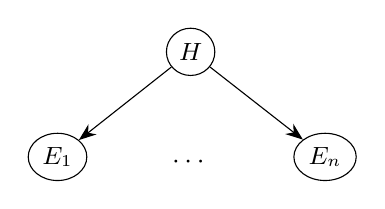
\begin{tikzpicture}[bn]
    \node[var] (H) {$H$};
    \node[var, below left=of H] (E1) {$E_1$};
    \node[below=of H] (dots) {$\cdots$};
    \node[var, below right=of H] (En) {$E_n$};
    \draw[->] (H) -- (E1); \draw[->] (H) -- (En);
  \end{tikzpicture}
  \end{center}
}

\mprop{Parametri del Naive Bayes}{
  Se $H$ ha $k$ valori e ogni $E_i$ ne ha al più $r$, il modello richiede
  \[
    (k-1) + n\,k\,(r-1)
  \]
  parametri liberi: \textbf{lineare} in $n$ (per $k, r$ fissati).
  Es.\ dentista: $H = \mathit{Cavity}$, $E_1 = \mathit{Toothache}$,
  $E_2 = \mathit{Catch}$: $1 + 2\cdot2\cdot1 = 5$.
}

\nt{ Si chiama ``naive'' perché viene usato anche quando
  l'indipendenza condizionata degli effetti \emph{non} è vera; nonostante ciò
  funziona spesso sorprendentemente bene (es.\ classificazione di testi/spam).
}

\chapter{Reti bayesiane}

% =====================================================================
\section{Rappresentazione e semantica}
% =====================================================================

% =====================================================================
\subsection{Sintassi}
% =====================================================================

\subsubsection{Grafi diretti aciclici}

\dfn{Grafo diretto aciclico (DAG)}{
  Un \textbf{DAG} è un grafo con archi orientati in cui è impossibile partire da
  un nodo e tornarci seguendo il verso delle frecce (nessun ciclo
  \emph{diretto}). Un triangolo $A\to B$, $A\to C$, $B\to C$ è un DAG: il grafo
  non orientato sottostante ha un ciclo, ma seguendo le frecce non si torna mai
  indietro. $A\to B\to C\to A$ invece non lo è.
}

\mlenma{Ordinamento topologico}{
  Ogni DAG finito ammette un \textbf{ordinamento topologico}: un ordinamento
  $X_1,\dots,X_n$ dei nodi tale che ogni arco va da un nodo precedente a uno
  successivo, cioè $\Par(X_i) \subseteq \{X_1,\dots,X_{i-1}\}$.
}
\pf{Dimostrazione}{
  Un DAG finito non vuoto ha almeno un nodo senza archi entranti (una
  \emph{radice}): altrimenti, risalendo gli archi all'indietro da un nodo
  qualunque, dopo al più $n$ passi si rivisita un nodo, trovando un ciclo
  diretto. Si mette la radice per prima, la si rimuove (il grafo resta un DAG) e
  si procede per induzione sui nodi rimanenti.
}

\nt{
  L'aciclicità serve proprio a questo: permette di ordinare le variabili in modo
  che la probabilità di ogni nodo sia specificata solo in funzione di variabili
  che vengono prima.
}

\subsubsection{Definizione di rete bayesiana}

\dfn{Rete bayesiana (sintassi)}{
  Una \textbf{rete bayesiana} su variabili $X_1,\dots,X_n$ consiste di:
  \begin{itemize}
    \item un \textbf{nodo} per ogni variabile;
    \item un \textbf{DAG} sui nodi;
    \item per ogni nodo, una \textbf{distribuzione condizionata locale}
      $\Pb(X_i \mid \Par(X_i))$.
  \end{itemize}
  Un arco $X_j \to X_i$ significa che $X_j$ è \textbf{genitore} di $X_i$:
  rappresenta una dipendenza probabilistica diretta (``influenza
  direttamente''), \textbf{non} necessariamente una relazione causale.
  La topologia codifica asserzioni di indipendenza condizionata.
}

\dfn{Tabella di probabilità condizionata (CPT)}{
  Se le variabili sono discrete, ogni distribuzione locale è una
  \textbf{CPT}: per ogni combinazione di valori dei genitori, una riga dà una
  distribuzione sui valori di $X_i$. Un nodo senza genitori ha come CPT la sua
  probabilità a priori.
}

\subsubsection{Esempi}

\ex{Rete del dentista}{
  \begin{center}
  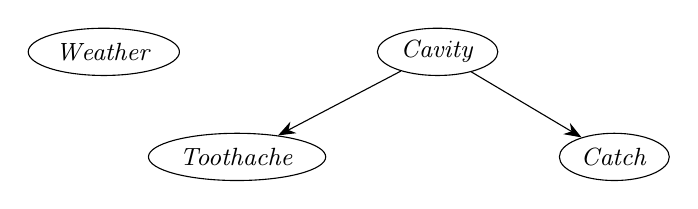
\begin{tikzpicture}[bn]
    \node[var] (W) {$\mathit{Weather}$};
    \node[var, right=25mm of W] (C) {$\mathit{Cavity}$};
    \node[var, below left=of C] (T) {$\mathit{Toothache}$};
    \node[var, below right=of C] (K) {$\mathit{Catch}$};
    \draw[->] (C) -- (T); \draw[->] (C) -- (K);
  \end{tikzpicture}
  \end{center}
  $\mathit{Weather}$ è indipendente dalle altre; $\mathit{Toothache}$ e
  $\mathit{Catch}$ sono condizionatamente indipendenti dato $\mathit{Cavity}$.
}

\ex{Rete dell'allarme (Burglary network)}{
  Sono al lavoro; il vicino John chiama dicendo che l'allarme suona; la vicina
  Mary non chiama. L'allarme può scattare per un furto, ma a volte anche per un
  piccolo terremoto. Vogliamo
  $P(\mathit{Burglary}\mid\mathit{JohnCalls}=\mathit{true},\mathit{MaryCalls}=\mathit{false})$.
  \begin{center}
  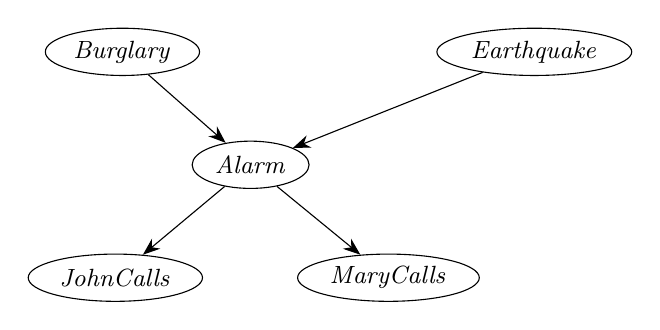
\begin{tikzpicture}[bn]
    \node[var] (B) {$\mathit{Burglary}$};
    \node[var, right=30mm of B] (E) {$\mathit{Earthquake}$};
    \node[var, below right=10mm and 4mm of B] (A) {$\mathit{Alarm}$};
    \node[var, below left=10mm and 4mm of A] (J) {$\mathit{JohnCalls}$};
    \node[var, below right=10mm and 4mm of A] (M) {$\mathit{MaryCalls}$};
    \draw[->] (B) -- (A); \draw[->] (E) -- (A);
    \draw[->] (A) -- (J); \draw[->] (A) -- (M);
  \end{tikzpicture}
  \end{center}
  \begin{center}
  \small
  \begin{tabular}{c}
    $P(b)$ \\ \midrule $0.001$
  \end{tabular}\qquad
  \begin{tabular}{c}
    $P(e)$ \\ \midrule $0.002$
  \end{tabular}\qquad
  \begin{tabular}{cc|c}
    $B$ & $E$ & $P(a\mid B,E)$ \\ \midrule
    T & T & 0.95 \\ T & F & 0.94 \\ F & T & 0.29 \\ F & F & 0.001
  \end{tabular}\qquad
  \begin{tabular}{c|c}
    $A$ & $P(j\mid A)$ \\ \midrule T & 0.90 \\ F & 0.05
  \end{tabular}\qquad
  \begin{tabular}{c|c}
    $A$ & $P(m\mid A)$ \\ \midrule T & 0.70 \\ F & 0.01
  \end{tabular}
  \end{center} Le probabilità \emph{riassumono} un insieme potenzialmente
  infinito di circostanze: Mary che ascolta musica alta e non sente l'allarme,
  John che confonde il telefono con l'allarme, ecc. --- senza modellarle.
}

\subsection{Semantica globale}

\subsubsection{Fattorizzazione della congiunta}

\dfn{Semantica globale di una rete bayesiana}{
  Le distribuzioni locali definiscono la \textbf{distribuzione congiunta
  completa} come loro prodotto:
  \[
    P(x_1,\dots,x_n) = \prod_{i=1}^{n} P\big(x_i \mid \mathit{pa}_i\big),
  \]
  dove $\mathit{pa}_i$ sono i valori assegnati ai genitori di $X_i$
  nell'assegnazione completa $(x_1,\dots,x_n)$.
  \textbf{Lettura}: per un'assegnazione completa si sceglie una entry dalla CPT di
  ogni nodo e si moltiplicano.
}

\ex{Un evento atomico nella rete dell'allarme}{
  ``L'allarme suona, John e Mary chiamano, nessun furto né terremoto'':
  \begin{align*}
    P(j, m, a, \neg b, \neg e) &= P(j\mid a)\,P(m\mid a)\,P(a\mid\neg b,\neg e)\,P(\neg b)\,P(\neg e) \\
    &= 0.9 \cdot 0.7 \cdot 0.001 \cdot 0.999 \cdot 0.998 \approx 0.00063 .
  \end{align*}
  La rete ricostruisce ogni evento atomico dalle CPT senza memorizzare la congiunta.
}

\nt{ Ne segue che una rete bayesiana può rispondere a
  \emph{qualsiasi} query, sommando le entrate rilevanti della congiunta
  (inferenza per enumerazione, eventualmente reso efficiente --- prossimo argomento).
}

\subsubsection{Compattezza}

\mprop{Compattezza}{
  Una CPT per una $X_i$ booleana con $k$ genitori booleani ha $2^k$ righe, ognuna
  con un solo numero $p$ (l'altro è $1-p$). Se ogni nodo ha al più $k$ genitori,
  la rete richiede
  \[
    O(n \cdot 2^k) \quad\text{numeri, contro}\quad O(2^n) \text{ della congiunta completa:}
  \]
  cresce \textbf{linearmente} in $n$.
}

\ex{Conteggio dei parametri}{
  \begin{itemize}
    \item Rete dell'allarme: $1+1+4+2+2 = 10$ numeri contro $2^5 - 1 = 31$.
    \item Rete dello studente (sotto): $1+1+8+2+3 = 15$ contro $2^4\cdot 3 - 1 = 47$.
    \item $n=30$ nodi con $k=5$ genitori: $30\cdot 2^5 = 960$
      numeri contro $2^{30} \approx 10^9$.
  \end{itemize}
}

\dfn{Sistema localmente strutturato}{
  Un sistema è \textbf{localmente strutturato} (o \emph{sparso}) se ogni
  componente interagisce direttamente solo con un numero limitato di altre
  componenti. Le reti bayesiane sono compatte proprio per questa proprietà,
  tipica dei domini reali; la complessità cresce linearmente invece che
  esponenzialmente.
}

\subsection{Pattern di ragionamento}

L'inferenza \textbf{non} deve seguire il verso delle frecce: si può ragionare
dalle cause agli effetti, dalle osservazioni alle spiegazioni, o tra spiegazioni
alternative.

\subsubsection{La rete dello studente}

\ex{La rete dello studente}{
  Il voto ($\mathit{Grade}$) dipende dall'intelligenza dello studente
  ($\mathit{Intelligence}$) e dalla difficoltà del corso ($\mathit{Difficulty}$).
  Il punteggio $\mathit{SAT}$ è correlato all'intelligenza. Il professore scrive
  la lettera di referenze ($\mathit{Letter}$) guardando solo il voto.
  \begin{center}
  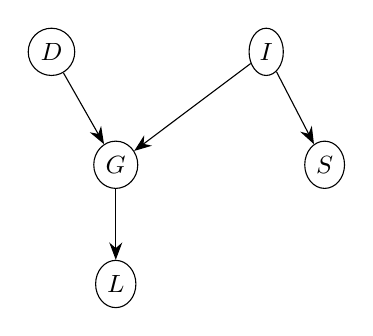
\begin{tikzpicture}[bn]
    \node[var] (D) {$D$};
    \node[var, right=22mm of D] (I) {$I$};
    \node[var, below right=10mm and 4mm of D] (G) {$G$};
    \node[var, below right=10mm and 4mm of I] (S) {$S$};
    \node[var, below=of G] (L) {$L$};
    \draw[->] (D) -- (G); \draw[->] (I) -- (G); \draw[->] (I) -- (S); \draw[->] (G) -- (L);
  \end{tikzpicture}
  \end{center}
}

\subsubsection{Tre tipi di ragionamento}

\dfn{Ragionamento predittivo (causale)}{
  Si predice un effetto a partire da cause note, nel verso delle frecce.
  Es.\ $P(\mathit{Letter}=\mathit{strong})$: $0.50$ a priori; $0.39$ se
  $I = \mathit{normal}$; $0.51$ se inoltre $D = \mathit{easy}$.
}

\dfn{Ragionamento diagnostico (evidenziale)}{
  Si inferisce una spiegazione non osservata a partire dall'evidenza, contro il
  verso delle frecce. Es.\ $P(I = \mathit{superior})$: $0.30$ a priori; $0.08$
  se $G = \mathit{poor}$; $0.14$ se $L = \mathit{weak}$; $0.08$ con entrambi;
  $0.58$ se si aggiunge $S = \mathit{high}$.
}

\dfn{Ragionamento intercausale (explaining away)}{
  Osservato un effetto comune, l'evidenza su una causa \textbf{modifica} la
  credenza nell'altra causa. Es.\ con $G = \mathit{poor}$: $P(I=\mathit{superior})
  = 0.08$; se si scopre anche $D = \mathit{hard}$ sale a $0.11$ (il voto basso è
  ``spiegato'' dalla difficoltà). Con $G = \mathit{good}$: $0.17$, e con $D =
  \mathit{hard}$ sale a $0.34$.
}

\subsection{Flusso di influenza e d-separazione}

\subsubsection{Trail e pattern di base}

\dfn{Trail}{
  Un \textbf{trail} è un cammino nella rete che segue nodi connessi
  \textbf{ignorando il verso degli archi}: $X_1 \rightleftharpoons \cdots
  \rightleftharpoons X_n$.
}

Per capire se due variabili possono dipendere probabilisticamente data
l'evidenza, ci si chiede se esiste un \textbf{trail attivo} tra loro.
Il caso base è il trail di due archi $X \rightleftharpoons Z \rightleftharpoons Y$:

\dfn{I tre pattern di base}{
  \begin{center}
  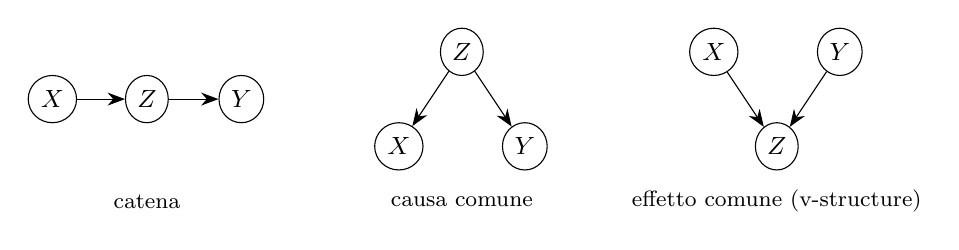
\begin{tikzpicture}[bn]
    % catena
    \node[var] (x1) at (0,0) {$X$}; \node[var] (z1) at (1.2,0) {$Z$}; \node[var] (y1) at (2.4,0) {$Y$};
    \draw[->] (x1) -- (z1); \draw[->] (z1) -- (y1);
    \node[font=\footnotesize] at (1.2,-1.3) {catena};
    % causa comune
    \node[var] (z2) at (5.2,0.6) {$Z$}; \node[var] (x2) at (4.4,-0.6) {$X$}; \node[var] (y2) at (6.0,-0.6) {$Y$};
    \draw[->] (z2) -- (x2); \draw[->] (z2) -- (y2);
    \node[font=\footnotesize] at (5.2,-1.3) {causa comune};
    % effetto comune
    \node[var] (x3) at (8.4,0.6) {$X$}; \node[var] (y3) at (10.0,0.6) {$Y$}; \node[var] (z3) at (9.2,-0.6) {$Z$};
    \draw[->] (x3) -- (z3); \draw[->] (y3) -- (z3);
    \node[font=\footnotesize] at (9.2,-1.3) {effetto comune (v-structure)};
  \end{tikzpicture}
  \end{center}
  \begin{center}
  \begin{tabular}{lccc}
    \toprule
    & Catena $X\to Z\to Y$ & Causa comune $X\leftarrow Z\to Y$ & Effetto comune $X\to Z\leftarrow Y$ \\
    \midrule
    Ruolo di $Z$ & non-collider & non-collider & \textbf{collider} \\
    $Z$ non osservato & attivo & attivo & \textbf{bloccato} \\
    $Z$ osservato & bloccato & bloccato & \textbf{attivo} \\
    \bottomrule
  \end{tabular}
  \end{center}
  Osservare un nodo intermedio ordinario \textbf{blocca} il trail; osservare un
  collider (o un suo discendente) lo \textbf{apre}.
}

\ex{Intuizioni sui tre pattern}{
  \begin{itemize}
    \item \textbf{Catena} $\mathit{Rain}\to\mathit{WetGrass}\to\mathit{SlipperyPath}$:
      se non so se l'erba è bagnata, sapere che è piovuto cambia la credenza
      sul sentiero scivoloso; se so che l'erba è bagnata, la pioggia non aggiunge
      nulla: $\cind{\mathit{Rain}}{\mathit{SlipperyPath}}{\mathit{WetGrass}}$.
    \item \textbf{Causa comune}
      $\mathit{IceCreamSales}\leftarrow\mathit{HotWeather}\to\mathit{SunglassesSales}$:
      vendite alte di gelati rendono più plausibile il caldo e quindi le vendite di
      occhiali; noto il caldo, i gelati non dicono più nulla sugli occhiali.
    \item \textbf{Effetto comune}
      $\mathit{Burglary}\to\mathit{Alarm}\leftarrow\mathit{Earthquake}$:
      furto e terremoto sono indipendenti; osservato l'allarme, confermare il
      furto rende meno necessario il terremoto per spiegarlo (\emph{explaining away}).
  \end{itemize}
}

\subsubsection{Trail attivi e d-separazione}

\dfn{Trail attivo}{
  Sia $\mathbf{Z}$ un insieme di variabili osservate. Un trail
  $X_1 \rightleftharpoons \cdots \rightleftharpoons X_n$ è \textbf{attivo dato
  $\mathbf{Z}$} se ogni nodo interno $X_i$ soddisfa:
  \begin{itemize}
    \item se $X_{i-1} \to X_i \leftarrow X_{i+1}$ (collider), allora $X_i$
      \textbf{o un suo discendente} appartiene a $\mathbf{Z}$;
    \item altrimenti (non-collider), $X_i \notin \mathbf{Z}$.
  \end{itemize}
}

\dfn{Nodo bloccato}{
  Dato $\mathbf{Z}$, un nodo intermedio di un trail è \textbf{bloccato} se:
  \begin{itemize}
    \item è il centro di una v-structure \emph{non marcata} (collider tale che né
      esso né alcun discendente è osservato); oppure
    \item è un non-collider che appartiene a $\mathbf{Z}$.
  \end{itemize}
  Un trail è attivo se e solo se nessun suo nodo interno è bloccato.
}

\dfn{d-separazione}{
  Due insiemi di nodi $\mathbf{X}$, $\mathbf{Y}$ sono \textbf{d-separati} dato
  $\mathbf{Z}$ se non esiste alcun trail attivo, dato $\mathbf{Z}$, tra un
  $X\in\mathbf{X}$ e un $Y\in\mathbf{Y}$.
}

\thm{Correttezza della d-separazione}{
  Per ogni distribuzione $P$ rappresentata dalla rete bayesiana:
  \[
    \mathbf{X} \text{ e } \mathbf{Y} \text{ d-separati dato } \mathbf{Z}
    \;\Longrightarrow\;
    P \models \cind{\mathbf{X}}{\mathbf{Y}}{\mathbf{Z}} .
  \]
}

\nt{
  Il viceversa vale solo in senso debole: se $\mathbf{X}$ e $\mathbf{Y}$
  \emph{non} sono d-separati, esiste \emph{qualche} distribuzione compatibile
  con il grafo in cui sono dipendenti (ma per CPT particolari potrebbero essere
  indipendenti ``per caso''). La d-separazione legge le indipendenze
  \emph{garantite dalla struttura}.
}

\mprop{Algoritmo per verificare $\cind{X}{Y}{\mathbf{Z}}$}{
  \begin{enumerate}
    \item Percorri il grafo dal basso verso l'alto \textbf{marcando} tutti i nodi
      in $\mathbf{Z}$ o che hanno discendenti in $\mathbf{Z}$.
    \item Percorri il grafo da $X$ verso $Y$, fermandoti quando incontri un nodo
      bloccato.
    \item Se non puoi raggiungere $Y$, allora $X$ e $Y$ sono indipendenti dato $\mathbf{Z}$.
  \end{enumerate}
}

\subsubsection{Esempi}

\ex{d-separazione guidata}{
  Rete: $A\to C$, $A\to D$, $B\to C$, $B\to D$, $C\to E$, $E\to F$, $D\to F$,
  $F\to H$, $H\to J$. Ci chiediamo se $C$ e $D$ sono d-separati.
  \begin{center}
  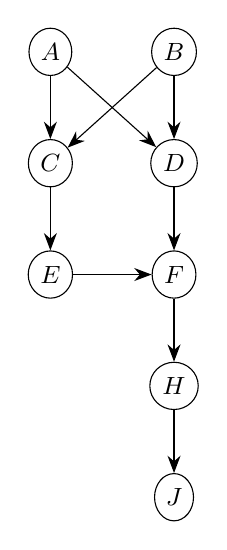
\begin{tikzpicture}[bn, node distance=8mm and 10mm]
    \node[var] (A) {$A$}; \node[var, right=of A] (B) {$B$};
    \node[var, below=of A] (C) {$C$}; \node[var, below=of B] (D) {$D$};
    \node[var, below=of C] (E) {$E$}; \node[var, below=of D] (F) {$F$};
    \node[var, below=of F] (H) {$H$}; \node[var, below=of H] (J) {$J$};
    \draw[->] (A) -- (C); \draw[->] (A) -- (D); \draw[->] (B) -- (C); \draw[->] (B) -- (D);
    \draw[->] (C) -- (E); \draw[->] (E) -- (F); \draw[->] (D) -- (F);
    \draw[->] (F) -- (H); \draw[->] (H) -- (J);
  \end{tikzpicture}
  \end{center}
  Trail rilevanti: $T_1: C\leftarrow A\to D$; \ $T_2: C\leftarrow B\to D$; \
  $T_3: C\to E\to F\leftarrow D$ (collider in $F$).
  \begin{enumerate}
    \item $\mathbf{Z}=\emptyset$: \textbf{dipendenti} ($T_1$, $T_2$ attivi; $T_3$
      bloccato in $F$).
    \item $\mathbf{Z}=\{A\}$: \textbf{dipendenti} ($T_1$ bloccato, ma $T_2$ attivo).
    \item $\mathbf{Z}=\{A,B\}$: \textbf{indipendenti} ($T_1,T_2$ bloccati;
      $T_3$ bloccato nel collider $F$ non osservato).
    \item $\mathbf{Z}=\{A,B,J\}$: \textbf{dipendenti} ($J$ è discendente di $F$:
      osservarlo apre il collider, $T_3$ diventa attivo).
    \item $\mathbf{Z}=\{A,B,E,J\}$: \textbf{indipendenti} ($T_3$ è aperto in $F$
      ma bloccato dal non-collider osservato $E$).
  \end{enumerate}
}

\ex{Indipendenze della rete dello studente}{
  Leggendo la d-separazione sul grafo $D\to G\leftarrow I\to S$, $G\to L$:
  \[
    \cind{L}{\{I,D,S\}}{G},\quad
    \cind{S}{\{G,D,L\}}{I},\quad
    \cind{G}{S}{I},\quad
    I \indip D,\quad
    D \indip \{I, S\}.
  \]
}

\subsection{Semantica locale e Markov blanket}

\subsubsection{Proprietà di Markov locale}

\dfn{Semantica locale (proprietà di Markov locale)}{
  Ogni nodo $X$ è condizionatamente indipendente dai suoi
  \textbf{non-discendenti}, dati i suoi \textbf{genitori}:
  \[
    \cind{X}{\big(\mathit{NonDescendants}(X) \setminus \Par(X)\big)}{\Par(X)} .
  \]
  Per valutare quanto è probabile un nodo basta conoscere i genitori diretti. Es.\
  $\cind{\mathit{JohnCalls}}{\mathit{Burglary}}{\mathit{Alarm}}$.
}

\mlenma{Insiemi ancestrali}{
  Sia $\mathbf{A}$ un insieme di nodi \textbf{ancestrale} (chiuso rispetto ai
  genitori: se $X\in\mathbf{A}$ allora $\Par(X)\subseteq\mathbf{A}$). Se vale la
  semantica globale, allora
  \[
    P(\mathbf{a}) = \prod_{X_i \in \mathbf{A}} P(x_i \mid \mathit{pa}_i).
  \]
}
\pf{Dimostrazione}{
  Si sommano via i nodi fuori da $\mathbf{A}$ in ordine topologico
  \emph{inverso}. Ad ogni passo il nodo eliminato $X_k$ è una foglia rispetto ai
  nodi rimasti, quindi compare in un solo fattore, la sua CPT, e
  $\sum_{x_k} P(x_k\mid\mathit{pa}_k) = 1$. Nessun nodo di $\mathbf{A}$ ha come
  genitore un nodo eliminato (perché $\mathbf{A}$ è ancestrale), quindi i
  fattori di $\mathbf{A}$ restano intatti.
}

\thm{Semantica locale $\Leftrightarrow$ semantica globale}{
  Per un DAG $G$ e una distribuzione $P$ sulle sue variabili, sono equivalenti:
  \begin{enumerate}[label=(\roman*)]
    \item $P$ si fattorizza secondo $G$: $P(x_1,\dots,x_n) = \prod_i P(x_i\mid\mathit{pa}_i)$;
    \item $P$ soddisfa la proprietà di Markov locale per ogni nodo di $G$.
  \end{enumerate}
}
\pf{Dimostrazione}{
  \textbf{(ii)$\Rightarrow$(i).} Si prende un ordinamento topologico (Lemma
  sull'ordinamento topologico) e si applica la chain rule:
  $P(x_1,\dots,x_n) = \prod_i P(x_i \mid x_1,\dots,x_{i-1})$. I predecessori
  $X_1,\dots,X_{i-1}$ sono tutti non-discendenti di $X_i$ e contengono
  $\Par(X_i)$; per la proprietà locale
  $P(x_i\mid x_1,\dots,x_{i-1}) = P(x_i\mid\mathit{pa}_i)$.

  \textbf{(i)$\Rightarrow$(ii).} Sia $\mathbf{N}$ l'insieme dei non-discendenti
  di $X$. L'insieme $\mathbf{A} = \mathbf{N}\cup\{X\}$ è ancestrale: i genitori
  di $X$ non sono suoi discendenti, e se un genitore di $Y\in\mathbf{N}$ fosse
  discendente di $X$, lo sarebbe anche $Y$. Per il lemma sugli insiemi ancestrali,
  \[
    P(x, \mathbf{n}) = P(x\mid\mathit{pa}_X)\prod_{Y\in\mathbf{N}} P(y\mid\mathit{pa}_Y),
  \]
  e i fattori su $\mathbf{N}$ non contengono $x$. Quindi
  \[
    P(x\mid\mathbf{n}) = \frac{P(x\mid\mathit{pa}_X)\prod_{\mathbf{N}}(\cdots)}
    {\sum_{x'}P(x'\mid\mathit{pa}_X)\prod_{\mathbf{N}}(\cdots)} = P(x\mid\mathit{pa}_X),
  \]
  che dipende da $\mathbf{n}$ solo attraverso $\mathit{pa}_X$.
}

\subsubsection{Markov blanket}

\dfn{Markov blanket}{
  Il \textbf{Markov blanket} $\mathit{MB}(X)$ di un nodo $X$ è formato da:
  \begin{itemize}
    \item i \textbf{genitori} di $X$;
    \item i \textbf{figli} di $X$;
    \item gli \textbf{altri genitori dei figli} di $X$.
  \end{itemize}
  Es.\ $\mathit{MB}(\mathit{Alarm}) = \{\mathit{Burglary}, \mathit{Earthquake},
  \mathit{JohnCalls}, \mathit{MaryCalls}\}$ (qui i figli non hanno altri genitori).
}

\thm{Proprietà del Markov blanket}{
  Dato il suo Markov blanket, $X$ è condizionatamente indipendente da
  \emph{tutti} gli altri nodi della rete:
  \[
    \cind{X}{\big(\mathbf{V}\setminus(\{X\}\cup\mathit{MB}(X))\big)}{\mathit{MB}(X)} .
  \]
}
\pf{Dimostrazione}{
  Per la semantica globale, condizionando su tutte le altre variabili
  $\mathbf{v}_{-X}$:
  \[
    P(x \mid \mathbf{v}_{-X}) = \frac{\prod_i P(x_i\mid\mathit{pa}_i)}{\sum_{x'}\prod_i P(x_i\mid\mathit{pa}_i)\big|_{x=x'}} .
  \]
  I fattori che \emph{non} contengono $x$ si semplificano tra numeratore e
  denominatore. Restano solo la CPT di $X$ e quelle dei suoi figli $Y_j$:
  \[
    P(x \mid \mathbf{v}_{-X}) = \alpha\, P(x\mid\mathit{pa}_X)\prod_{Y_j\in\mathit{Children}(X)} P(y_j\mid\mathit{pa}_{Y_j}),
  \]
  che dipende solo da genitori di $X$, figli e genitori dei figli, cioè da $\mathit{MB}(X)$.
}

\nt{
  Il Markov blanket è il \textbf{più piccolo} insieme locale che contiene tutta
  l'informazione su un nodo disponibile nella rete. La formula nella
  dimostrazione è alla base dei metodi di campionamento come il \emph{Gibbs
  sampling}.
}

% =====================================================================
\section{Costruzione e apprendimento}
% =====================================================================

% =====================================================================
\subsection{Costruzione da un ordinamento}\label{sec:costruzione}
% =====================================================================

\subsubsection{Procedura e correttezza}

\dfn{Costruzione da un ordinamento}{
  \begin{enumerate}
    \item Scegli un ordinamento delle variabili $X_1,\dots,X_n$.
    \item Per $i = 1,\dots,n$:
      \begin{itemize}
        \item aggiungi $X_i$ alla rete;
        \item scegli $\Par(X_i) \subseteq \{X_1,\dots,X_{i-1}\}$ \textbf{minimale}
          tale che
          \[
            \cind{X_i}{\big(\{X_1,\dots,X_{i-1}\}\setminus\Par(X_i)\big)}{\Par(X_i)},
            \quad\text{cioè}\quad
            \Pb(X_i\mid X_1,\dots,X_{i-1}) = \Pb(X_i\mid\Par(X_i));
          \]
        \item aggiungi gli archi $\Par(X_i)\to X_i$ e scrivi la CPT $\Pb(X_i\mid\Par(X_i))$.
      \end{itemize}
  \end{enumerate}
}

\thm{Correttezza della costruzione}{
  La rete ottenuta è un DAG e rappresenta esattamente la congiunta:
  \[
    \Pb(X_1,\dots,X_n) = \prod_{i=1}^{n}\Pb(X_i\mid\Par(X_i)).
  \]
}
\pf{Dimostrazione}{
  \textbf{Aciclicità}: ogni arco va da $X_j$ a $X_i$ con $j<i$, quindi seguendo
  le frecce gli indici crescono strettamente e non si può tornare indietro.
  \textbf{Fattorizzazione}: per la chain rule
  $\Pb(X_1,\dots,X_n) = \prod_i \Pb(X_i\mid X_1,\dots,X_{i-1})$, e per la scelta
  dei genitori ogni fattore è uguale a $\Pb(X_i\mid\Par(X_i))$.
}

\nt{
  La procedura garantisce una fattorizzazione \emph{corretta} per qualsiasi
  ordinamento, ma \textbf{non} dice come ottenerne una \emph{compatta}. In
  pratica i genitori si scelgono con conoscenza del dominio (meglio se causale)
  oppure si imparano dai dati.
}

\subsubsection{Scelta dell'ordinamento}

\nt{
  \textbf{Perché un ordine causale è preferibile.} Ordinare dalle cause agli
  effetti di solito rende più facile identificare le indipendenze condizionate,
  stimare le probabilità richieste (le probabilità causali sono più naturali per
  un esperto) e ottenere una rete compatta con pochi genitori per nodo.
}

\ex{Ordinamento non causale: $M, J, A, B, E$}{
  \begin{itemize}
    \item $P(J\mid M) = P(J)$? \textbf{No} (se Mary chiama, è più probabile che
      l'allarme suoni e quindi che John chiami) $\Rightarrow$ $M\to J$.
    \item $P(A\mid J,M) = P(A\mid J)$? $P(A\mid J,M) = P(A)$? \textbf{No} $\Rightarrow$
      genitori $\{J, M\}$.
    \item $P(B\mid A,J,M) = P(B\mid A)$? \textbf{Sì}. \ $= P(B)$? \textbf{No}
      $\Rightarrow$ genitore $\{A\}$.
    \item $P(E\mid B,A,J,M) = P(E\mid A)$? \textbf{No}. \ $= P(E\mid A,B)$?
      \textbf{Sì} $\Rightarrow$ genitori $\{A,B\}$.
  \end{itemize}
  Parametri: $1 + 2 + 4 + 2 + 4 = 13$, contro i $10$ dell'ordine causale. Inoltre alcune CPT sono innaturali da stimare (es.\
  $P(E\mid B,A)$); con l'ordine $M,J,E,B,A$ si arriva a $31$ parametri, tanti
  quanti la congiunta completa.
}

\ex{Perché un buon ordinamento conta}{
  Sapendo che $\cind{\mathit{MaryCalls}}{\mathit{JohnCalls}}{\mathit{Alarm}}$:
  \begin{itemize}
    \item ordine causale $A, M, J$:
      $P(A)P(M\mid A)P(J\mid A)$ $\Rightarrow$ $1+2+2 = 5$ parametri;
    \item ordine $M, J, A$:
      $P(M)P(J\mid M)P(A\mid M,J)$ $\Rightarrow$ $1+2+4 = 7$ parametri.
  \end{itemize}
  Rappresentano la stessa distribuzione, ma l'ordine causale rende esplicita
  l'indipendenza e usa meno parametri.
}

\nt{
  \textbf{Direzione di un arco.} Poiché $P(M,J) = P(M)P(J\mid M) = P(J)P(M\mid J)$,
  sia $M\to J$ sia $J\to M$ sono fattorizzazioni valide della stessa dipendenza,
  con CPT diverse. Le due frecce \textbf{non} possono coesistere: formerebbero un
  ciclo, e $P(M\mid J)\,P(J\mid M) \neq P(M,J)$ in generale --- non c'è un
  ordine in cui specificare una variabile prima dell'altra. Una rete bayesiana
  richiede una fattorizzazione non circolare.
}

\nt{
  \textbf{Obiettivo.} Non si cerca di rendere ogni variabile indipendente; si
  cerca un ordinamento e un \emph{piccolo} insieme di genitori diretti per ogni
  variabile, tali che le altre variabili precedenti non aggiungano informazione
  una volta noti i genitori.
}

\subsection{Esempi di modellazione}

\subsubsection{Monty Hall}

\ex{Il problema di Monty Hall}{
  Siamo in un quiz televisivo davanti a tre porte chiuse; dietro una c'è un
  premio. Scegliamo la porta di sinistra. Il conduttore, che sa dov'è il premio,
  apre la porta centrale mostrando che è vuota. Ci viene offerto di cambiare
  scelta. Conviene?

  \textbf{Variabili}: $\mathit{Prize}, \mathit{Choice}, \mathit{HostOpens}
  \in\{\mathit{left},\mathit{middle},\mathit{right}\}$.
  \textbf{Conoscenza del dominio}: il conduttore non apre mai né la porta scelta
  né quella col premio; se può scegliere tra due porte, sceglie a caso.
  \begin{center}
  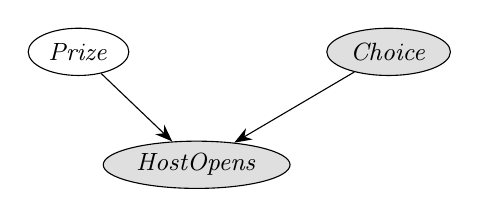
\begin{tikzpicture}[bn]
    \node[var] (P) {$\mathit{Prize}$};
    \node[obs, right=25mm of P] (C) {$\mathit{Choice}$};
    \node[obs, below right=10mm and 2mm of P] (H) {$\mathit{HostOpens}$};
    \draw[->] (P) -- (H); \draw[->] (C) -- (H);
  \end{tikzpicture}
  \end{center}
  La struttura è un \textbf{collider}: osservare $\mathit{HostOpens}$ rende
  $\mathit{Prize}$ dipendente da $\mathit{Choice}$, ed è questo che rende
  informativa la porta aperta.

  \textbf{Evidenza}: $\mathit{Choice}=\mathit{left}$, $\mathit{HostOpens}=\mathit{middle}$.
  \begin{center}
  \begin{tabular}{lccc}
    \toprule
    $\mathit{Prize}$ & prior & $P(\mathit{HostOpens}=\mathit{middle}\mid\cdot)$ & prodotto \\
    \midrule
    $\mathit{left}$ & $1/3$ & $1/2$ & $1/6$ \\
    $\mathit{middle}$ & $1/3$ & $0$ & $0$ \\
    $\mathit{right}$ & $1/3$ & $1$ & $1/3$ \\
    \bottomrule
  \end{tabular}
  \end{center}
  Normalizzando ($1/6 + 0 + 1/3 = 1/2$):
  $P(\mathit{Prize}=\mathit{left}\mid\mathbf{e}) = 1/3$,
  $P(\mathit{Prize}=\mathit{right}\mid\mathbf{e}) = 2/3$. \textbf{Conviene cambiare.}
}

\nt{
  Un'osservazione aggiorna le credenze sulle cause non osservate quando
  l'osservazione \emph{dipende} da quelle cause.
}

\subsubsection{Diagnosi dell'auto}

\ex{Diagnosi dell'auto}{
  Evidenza iniziale: $\mathit{CarWon'tStart}$. I nodi si dividono in:
  sintomo osservato; variabili \textbf{testabili} (luci, indicatore dell'olio,
  indicatore della benzina, astina); guasti \textbf{riparabili} (batteria
  scarica, alternatore rotto, cinghia rotta, niente olio/benzina, tubo
  ostruito, motorino rotto); variabili \textbf{nascoste} intermedie (batteria
  morta, non carica, ecc.). Le variabili nascoste aumentano il numero di nodi ma
  riducono drasticamente i parametri.
}

\subsection{Apprendere una rete dai dati}

\subsubsection{Apprendere la struttura}

\dfn{Structure learning}{
  Quando la conoscenza del dominio non basta a fissare il grafo, si usano i dati
  per apprendere una struttura plausibile.
  \begin{itemize}
    \item \textbf{Metodi constraint-based}: (1) test statistici di indipendenza
      condizionata; (2) si deduce quali archi devono mancare o possono esserci;
      (3) si cerca un grafo compatibile con questi vincoli.
    \item \textbf{Metodi score-based}: (1) si definisce uno score che misura quanto
      una rete spiega i dati penalizzando la complessità; (2) si cerca la struttura
      con score migliore.
  \end{itemize}
}

\nt{
  \textbf{Limite}: strutture diverse possono spiegare ugualmente bene i dati
  osservazionali; i dati da soli non determinano in generale la direzione causale
  di ogni arco. La conoscenza del dominio fornisce vincoli (ordine temporale,
  relazioni causali vietate o richieste). Fissata la struttura, le CPT si stimano
  dai dati o si chiedono agli esperti.
}

\subsubsection{Apprendere i parametri}

\nt{
  Una rete bayesiana specifica una \textbf{struttura} ($\Par(X_i)$, da
  conoscenza del dominio o appresa) e dei \textbf{modelli locali}
  ($\Pb(X_i\mid\Par(X_i))$, specificati da probabilità o parametri). Da dove
  vengono i numeri?
}

\dfn{Parameter learning}{
  Data la struttura, il \textbf{parameter learning} (forma di \emph{density
  estimation}) stima le distribuzioni $\Pb(X_i\mid\Par(X_i))$. Fonti possibili:
  \begin{itemize}
    \item \textbf{esperti del dominio}: probabilità elicitate;
    \item \textbf{modelli meccanicistici}: parametri da equazioni fisiche o del dominio;
    \item \textbf{dati}: parametri stimati dalle osservazioni.
  \end{itemize}
  Approcci: \textbf{maximum likelihood} (parametri che rendono i dati più
  probabili), \textbf{apprendimento bayesiano} (prior sui parametri + dati),
  \textbf{EM} (quando alcune variabili sono nascoste o mancano valori).
}

\mprop{Stima di massima verosimiglianza di una CPT}{
  Con dati completi, la stima ML di ogni entry di una CPT è la
  \textbf{frequenza relativa osservata}:
  \[
    \hat{P}(X_i = x \mid \Par(X_i) = \mathit{pa}) = \frac{N(X_i = x,\ \Par(X_i) = \mathit{pa})}{N(\Par(X_i) = \mathit{pa})} .
  \]
  Grazie alla fattorizzazione, la verosimiglianza si decompone e ogni CPT si
  stima \textbf{separatamente}.
}
\pf{Dimostrazione (caso booleano)}{
  Con $c$ casi positivi su $N$ con genitori $\mathit{pa}$, la verosimiglianza è
  $L(\theta) = \theta^{c}(1-\theta)^{N-c}$. Derivando il log:
  $\frac{c}{\theta} - \frac{N-c}{1-\theta} = 0 \Rightarrow \hat\theta = c/N$.
}

% =====================================================================
\subsection{Reti causali}
% =====================================================================

\subsubsection{Dalla dipendenza alla causalità}

\ex{Fuoco e fumo}{
  Le reti $\mathit{Fire}\to\mathit{Smoke}$ e $\mathit{Smoke}\to\mathit{Fire}$
  rappresentano esattamente la stessa congiunta:
  \[
    P(\mathit{Fire},\mathit{Smoke}) = P(\mathit{Fire})P(\mathit{Smoke}\mid\mathit{Fire})
    = P(\mathit{Smoke})P(\mathit{Fire}\mid\mathit{Smoke}).
  \]
  I dati osservazionali non le distinguono. Ma sono davvero equivalenti?
  Accendere un fumogeno non fa scoppiare un incendio.
}

\dfn{Rete causale}{
  Una \textbf{rete causale} è una rete bayesiana arricchita con assunzioni
  causali: è la sottoclasse di reti che ammette solo ordinamenti
  \textbf{causalmente compatibili}. Un arco $X_j\to X_i$ afferma che $X_j$ è un
  \textbf{input diretto del meccanismo} che genera $X_i$. Permette di ragionare
  su \textbf{interventi}, non solo su osservazioni.
}

\subsubsection{Equazioni strutturali}

\dfn{Equazione strutturale}{
  Per ogni variabile $X_i$, un'\textbf{equazione strutturale} specifica il
  meccanismo che ne produce il valore:
  \[
    X_i = f_i\big(\Par(X_i), U_i\big),
  \]
  dove $U_i$ è una variabile non modellata (termine di errore) che riassume gli
  altri fattori. L'arco $X_j\to X_i$ è presente \textbf{esattamente} quando
  $X_j$ è un argomento diretto di $f_i$.
  Es.\ $\mathit{Smoke} = f_{\mathit{Smoke}}(\mathit{Fire}, U_{\mathit{Smoke}})$,
  $\mathit{Fire} = f_{\mathit{Fire}}(U_{\mathit{Fire}})$.
}

\dfn{Invarianza (stabilità) dei meccanismi}{
  Un'equazione strutturale rappresenta un meccanismo causale
  \textbf{autonomo}: rimane invariato rispetto alle osservazioni e ai
  cambiamenti locali in altre parti dell'ambiente (es.\ irrigatore disattivato,
  prato coperto da una tenda: cambia un solo meccanismo, gli altri restano).
}

\ex{Il prato}{
  \begin{center}
  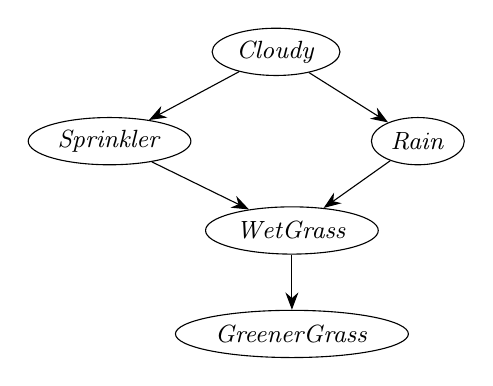
\begin{tikzpicture}[bn, node distance=7mm and 8mm]
    \node[var] (C) {$\mathit{Cloudy}$};
    \node[var, below left=of C] (S) {$\mathit{Sprinkler}$};
    \node[var, below right=of C] (R) {$\mathit{Rain}$};
    \node[var, below right=of S] (W) {$\mathit{WetGrass}$};
    \node[var, below=of W] (G) {$\mathit{GreenerGrass}$};
    \draw[->] (C) -- (S); \draw[->] (C) -- (R); \draw[->] (S) -- (W); \draw[->] (R) -- (W); \draw[->] (W) -- (G);
  \end{tikzpicture}
  \end{center}
  \[
    C = f_C(U_C),\quad R = f_R(C,U_R),\quad S = f_S(C,U_S),\quad
    W = f_W(S,R,U_W),\quad G = f_G(W,U_G).
  \]
}

\subsubsection{Interventi e operatore $\doop$}

\dfn{Operatore $\doop$ (intervento)}{
  $\doop(X = x)$ denota un \textbf{intervento} che fissa $X$ al valore $x$
  dall'esterno del sistema: l'equazione strutturale $X = f_X(\Par(X),U_X)$ viene
  \textbf{sostituita} da $X = x$.
  \textbf{Graficamente}: si rimuovono tutti gli archi \emph{entranti} in $X$
  (il suo valore non dipende più dalle cause usuali); gli archi \emph{uscenti}
  restano ($X$ influenza ancora le sue conseguenze).
}

\mprop{Fattorizzazione troncata}{
  In una rete causale, l'intervento $\doop(X_j = \hat{x})$ produce la
  distribuzione
  \[
    P\big(x_1,\dots,x_n \mid \doop(X_j=\hat{x})\big) =
    \begin{cases}
      \prod_{i\neq j} P(x_i\mid\mathit{pa}_i) & \text{se } x_j = \hat{x},\\
      0 & \text{altrimenti,}
    \end{cases}
  \]
  cioè si elimina dalla semantica globale il fattore $P(x_j\mid\mathit{pa}_j)$.
}

\ex{Osservare vs.\ intervenire}{
  \begin{itemize}
    \item $P(\mathit{WetGrass}\mid\mathit{Sprinkler}=\mathit{true})$: ``cosa credo
      sull'erba dopo aver \emph{osservato} che l'irrigatore è acceso?''
      L'osservazione dà informazione anche sulle sue cause ($\mathit{Cloudy}$, e
      quindi $\mathit{Rain}$): è probabile che non sia nuvoloso e quindi che non
      piova.
    \item $P(\mathit{WetGrass}\mid\doop(\mathit{Sprinkler}=\mathit{true}))$:
      ``cosa succederebbe all'erba se \emph{accendessi} l'irrigatore?''
      Si taglia l'arco $\mathit{Cloudy}\to\mathit{Sprinkler}$; $\mathit{Cloudy}$
      e $\mathit{Rain}$ mantengono la distribuzione a priori.
  \end{itemize}
  Le due risposte possono differire.
}

% =====================================================================
\section{Rappresentazioni compatte ed estensioni}
% =====================================================================

% =====================================================================
\subsection{Distribuzioni canoniche}
% =====================================================================

\subsubsection{Oltre le CPT}

\nt{
  \textbf{Limiti delle CPT}: una CPT cresce \textbf{esponenzialmente} col numero
  di genitori ($n$ genitori booleani $\Rightarrow$ $2^n$ righe; con 4 genitori
  già 16) e diventa \textbf{infinita} se il genitore o il figlio è continuo. Le
  CPT sono pratiche solo per nodi con pochi genitori discreti.
}

\dfn{Distribuzione canonica}{
  Una \textbf{distribuzione canonica} specifica $\Pb(X\mid\Par(X))$ tramite una
  \textbf{forma funzionale compatta} con pochi parametri, invece di elencare una
  entry per ogni combinazione dei valori dei genitori. La CPT è la
  rappresentazione generale; le distribuzioni canoniche sono rappresentazioni
  compatte per strutture ricorrenti. Esempi: nodi deterministici, noisy-OR,
  modelli ibridi.
}

\subsubsection{Nodi deterministici}

\dfn{Nodo deterministico}{
  Un nodo $X$ è \textbf{deterministico} se il suo valore è completamente
  determinato dai genitori:
  \[
    X = f(\Par(X)).
  \]
  Equivalentemente, noto $\Par(X) = \mathit{pa}$, la distribuzione condizionata
  assegna probabilità $1$ al valore $f(\mathit{pa})$ (nessuna incertezza).
}

\ex{Nodi deterministici}{
  \begin{itemize}
    \item \textbf{Booleano}: $\mathit{NorthAmerican} \equiv \mathit{Canadian}\lor\mathit{US}\lor\mathit{Mexican}$.
      Una regola logica sostituisce $2^3 = 8$ righe di CPT
      ($P = 0$ solo se $c = u = m = \mathit{false}$, altrimenti $1$): dimensione
      lineare nei genitori e nessun parametro da stimare.
    \item \textbf{Continuo}: il tasso di variazione del livello d'acqua
      $\dot{L} = \mathit{Inflow} + \mathit{Rainfall} - \mathit{Outflow} -
      \mathit{Evaporation}$. Con $I=5, R=2, O=3, E=1$: $\dot{L}=3$ con
      probabilità 1.
    \item Il prezzo migliore di un'auto è il $\min$ dei prezzi
      dei venditori.
  \end{itemize}
}

\subsubsection{Noisy-OR}

\nt{
  Un OR deterministico ($\mathit{Sneezing}\equiv\mathit{Flu}\lor\mathit{Allergy}\lor\mathit{Cold}$,
  oppure $\mathit{Alarm}\equiv\mathit{Burglary}\lor\mathit{Earthquake}$) è
  troppo forte: una causa attiva rende l'effetto più probabile, non certo (il
  sistema d'allarme può essere disattivato, un sensore può guastarsi).
}

\dfn{Noisy-OR}{
  Distribuzione canonica per un effetto booleano $Y$ con cause booleane
  $X_1,\dots,X_n$. Ogni causa attiva ha un meccanismo che può attivare $Y$, ma
  può \textbf{fallire} con \textbf{probabilità di inibizione} $q_i$. Assunzioni:
  \begin{itemize}
    \item tutte le cause possibili sono elencate (vedi \emph{leak node});
    \item l'inibizione di ciascuna causa è \textbf{indipendente} da quella delle altre.
  \end{itemize}
  L'effetto è falso solo se \textbf{tutte} le cause attive falliscono:
  \[
    P(Y=\mathit{false}\mid X_1,\dots,X_n) = \prod_{i\,:\,X_i=\mathit{true}} q_i,
    \qquad
    P(Y=\mathit{true}\mid X_1,\dots,X_n) = 1 - \prod_{i\,:\,X_i=\mathit{true}} q_i .
  \]
  $p_i = 1 - q_i$ è detta \textbf{link probability} (probabilità che $X_i$ da sola
  causi $Y$).
}

\dfn{Leak node}{
  Nel noisy-OR base, se nessuna causa modellata è attiva l'effetto non può
  verificarsi: $P(Y=\mathit{true}\mid X_1=\dots=X_n=\mathit{false}) = 0$. Per
  superare il limite si aggiunge un \textbf{leak node}: un genitore aggiuntivo
  \textbf{sempre attivo} che rappresenta tutte le cause non modellate.
}

\mprop{Parametri del noisy-OR}{
  Il noisy-OR specifica l'intera CPT di $Y$ con $n$ parametri (uno per causa)
  invece di $2^n$: il numero di parametri è \textbf{lineare} nel numero di genitori.
}

\ex{Allarme noisy-OR}{
  $p_B = 0.95$, $p_E = 0.30$ $\Rightarrow$ $q_B = 0.05$, $q_E = 0.70$.
  \begin{center}
  \begin{tabular}{cc|c}
    \toprule
    $B$ & $E$ & $P(\mathit{Alarm}=\mathit{true}\mid B,E)$ \\
    \midrule
    F & F & $0$ \\
    T & F & $p_B = 0.95$ \\
    F & T & $p_E = 0.30$ \\
    T & T & $1 - q_B q_E = 1 - 0.05\cdot0.70 = 0.965$ \\
    \bottomrule
  \end{tabular}
  \end{center}
}

\ex{Febbre (noisy-OR completo)}{
  $q_{\mathit{cold}} = 0.6$, $q_{\mathit{flu}} = 0.2$, $q_{\mathit{malaria}} = 0.1$:
  \begin{center}
  \begin{tabular}{ccc|cc}
    \toprule
    $\mathit{Cold}$ & $\mathit{Flu}$ & $\mathit{Malaria}$ & $P(\mathit{fever})$ & $P(\neg\mathit{fever})$ \\
    \midrule
    F & F & F & 0.0 & 1.0 \\
    F & F & T & 0.9 & 0.1 \\
    F & T & F & 0.8 & 0.2 \\
    F & T & T & 0.98 & $0.02 = 0.2\times0.1$ \\
    T & F & F & 0.4 & 0.6 \\
    T & F & T & 0.94 & $0.06 = 0.6\times0.1$ \\
    T & T & F & 0.88 & $0.12 = 0.6\times0.2$ \\
    T & T & T & 0.988 & $0.012 = 0.6\times0.2\times0.1$ \\
    \bottomrule
  \end{tabular}
  \end{center}
  Si danno solo i 3 valori $q_i$; le altre righe si calcolano.
}

\nt{
  \textbf{Caso reale: CPCS} (Pradhan et al., UAI 1994): rete bayesiana per la
  medicina interna con \textbf{448 nodi e 908 archi}, modellata con
  \textbf{noisy-MAX} (generalizzazione del noisy-OR a variabili multivalore) più
  probabilità di leak. Bastano
  8.254 valori invece dei 133.931.430 di una rete con CPT complete.
}

\subsection{Reti ibride}

\subsubsection{Discretizzazione o modelli parametrici}

\dfn{Rete bayesiana ibrida}{
  Una rete che contiene sia variabili \textbf{discrete} sia \textbf{continue}.
  Le distribuzioni locali possono combinare CPT, densità condizionate e altre
  forme parametriche compatte. Due opzioni:
  \begin{enumerate}
    \item \textbf{Discretizzazione}: si sostituiscono le variabili continue con
      intervalli e si usano CPT. Trade-off: pochi intervalli perdono informazione,
      molti producono CPT enormi.
    \item \textbf{Famiglie parametriche canoniche} con un numero finito di
      parametri, per (a) figlio continuo con genitori continui e/o discreti, e
      (b) figlio discreto con genitori continui.
  \end{enumerate}
}

\ex{Raccolto e acquisto}{
  Il costo ($\mathit{Cost}$, continuo) dipende dalla quantità raccolta
  ($\mathit{Harvest}$, continua) e dalla presenza di un sussidio
  ($\mathit{Subsidy?}$, discreta); il costo influenza la decisione di acquisto
  ($\mathit{Buys?}$, discreta). Servono $P(\mathit{Cost}\mid\mathit{Harvest},
  \mathit{Subsidy?})$ e $P(\mathit{Buys?}\mid\mathit{Cost})$.
  \begin{center}
  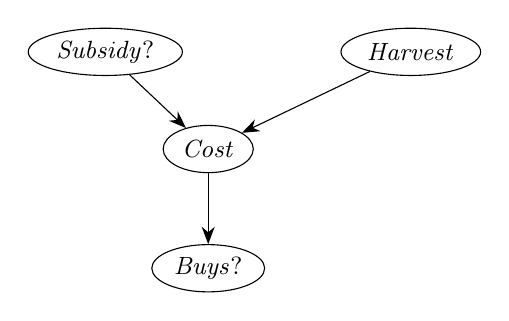
\begin{tikzpicture}[bn]
    \node[var] (S) {$\mathit{Subsidy?}$};
    \node[var, right=20mm of S] (H) {$\mathit{Harvest}$};
    \node[var, below right=8mm and 2mm of S] (C) {$\mathit{Cost}$};
    \node[var, below=of C] (B) {$\mathit{Buys?}$};
    \draw[->] (S) -- (C); \draw[->] (H) -- (C); \draw[->] (C) -- (B);
  \end{tikzpicture}
  \end{center}
}

\subsubsection{Figlio continuo: modello lineare gaussiano}

\dfn{Densità condizionata per un figlio continuo}{
  Per un figlio continuo $Y$, la distribuzione locale è una densità condizionata
  $p(y\mid\Par(Y))$: per ogni assegnazione fissata dei genitori è non negativa e
  integra a 1. Si definisce una densità separata per ogni assegnazione dei
  genitori \emph{discreti}; la densità può poi dipendere dai valori dei genitori
  \emph{continui}.
}

\dfn{Modello lineare gaussiano}{
  Il figlio ha distribuzione gaussiana la cui media varia \textbf{linearmente}
  con i genitori continui, con varianza fissa:
  \[
    \mathit{Cost} = a_t\,\mathit{Harvest} + b_t + \varepsilon_t,\qquad \varepsilon_t\sim\mathcal{N}(0,\sigma_t^2),
  \]
  cioè, fissati $\mathit{Harvest} = h$ e $\mathit{Subsidy?} = t$,
  \[
    \mathit{Cost}\mid(h,t) \sim \mathcal{N}(a_t h + b_t,\ \sigma_t^2),
    \qquad \mathbb{E}[\mathit{Cost}\mid h,t] = a_t h + b_t .
  \]
  $a_t$: come cambia il costo atteso al crescere del raccolto (pendenza,
  negativa perché più offerta abbassa il prezzo); $b_t$: intercetta;
  $\sigma_t^2$: incertezza residua. I parametri possono differire per
  $t = \mathit{true}$ e $t = \mathit{false}$.
}

\mprop{Reti lineari gaussiane}{
  \begin{itemize}
    \item Se \textbf{tutte} le variabili sono continue con distribuzioni lineari
      gaussiane, la congiunta è una \textbf{gaussiana multivariata}:
      $\Pb(X_1,\dots,X_n) = \mathcal{N}(\boldsymbol\mu,\boldsymbol\Sigma)$.
    \item Se ci sono anche genitori discreti (rete \textbf{gaussiana
      condizionata}), per ogni assegnazione $\mathbf{D}=\mathbf{d}$ delle discrete
      la distribuzione delle continue è una gaussiana multivariata.
    \item Se i genitori discreti non sono osservati si ottiene una
      \textbf{miscela di gaussiane}:
      $P(c\mid h) = \sum_{t} P(c\mid h,t)\,P(t)$.
  \end{itemize}
}

\nt{ L'assunzione di linearità implica che il costo diventi
  negativo per raccolti molto grandi: il modello è ragionevole solo su un range
  limitato di $\mathit{Harvest}$.
}

\subsubsection{Figlio discreto: probit e logit}

\dfn{Figlio discreto con genitore continuo}{
  Per un figlio discreto $Y$ con genitori continui $\mathbf{X}$ si specifica
  $P(Y=y\mid\mathbf{X}=\mathbf{x})$ per ogni $\mathbf{x}$; non potendo elencarli in
  una CPT finita, si usa una funzione con pochi parametri. Una regola
  deterministica ($\mathit{Buys?}$ sse $\mathit{Cost}<\mu$) è troppo rigida: serve
  una \textbf{soglia morbida} (soft threshold).
}

\dfn{Modello probit}{
  \[
    P(\mathit{Buys?}=\mathit{true}\mid\mathit{Cost}=c) = \Phi\!\left(\frac{\mu - c}{\sigma}\right),
  \]
  dove $\Phi$ è la funzione di ripartizione (CDF) della gaussiana standard,
  $\mu$ è il costo a cui la probabilità d'acquisto è $0.5$ e $\sigma$ controlla
  quanto è graduale la transizione.
}

\mprop{Giustificazione del probit}{
  Se il processo decisionale ha una soglia \emph{rigida} $T$ (``compro sse
  $c \le T$'') ma la posizione della soglia è soggetta a rumore gaussiano,
  $T\sim\mathcal{N}(\mu,\sigma^2)$, allora la probabilità d'acquisto è
  esattamente il modello probit.
}
\pf{Dimostrazione}{
  $P(\mathit{buys}\mid c) = P(T \ge c) = 1 - \Phi\!\left(\frac{c-\mu}{\sigma}\right)
  = \Phi\!\left(\frac{\mu-c}{\sigma}\right)$, per la simmetria
  $1-\Phi(z) = \Phi(-z)$ della gaussiana standard.
}

\dfn{Modello logit (logistico)}{
  Usa la funzione logistica (sigmoide) $1/(1+e^{-x})$:
  \[
    P(\mathit{Buys?}=\mathit{true}\mid\mathit{Cost}=c) = \frac{1}{1+\exp\!\left(-2\,\frac{-c+\mu}{\sigma}\right)} .
  \]
}

\nt{
  Probit e logit hanno forma simile, ma il logit ha \textbf{code più lunghe}.
  Il probit si adatta spesso meglio a situazioni reali; il logit è più comodo
  matematicamente ed è molto usato in machine learning.
}

\subsection{Reti bayesiane dinamiche}

\subsubsection{Stati e traiettorie}

\dfn{Stato, variabili template, traiettoria}{
  \begin{itemize}
    \item Lo \textbf{stato} del sistema al tempo $t$ è un insieme di variabili
      $X^{(t)} = \{X_1^{(t)},\dots,X_n^{(t)}\}$.
    \item Una \textbf{variabile template} $X_i$ denota la stessa quantità a ogni
      passo; $X_i^{(t)}$ è la sua istanza al tempo $t$.
    \item Una \textbf{traiettoria} è una sequenza completa di stati
      $\big(X^{(0)}, X^{(1)}, \dots, X^{(T)}\big)$.
  \end{itemize}
}

\dfn{Rete bayesiana dinamica (DBN)}{
  Una \textbf{DBN} è una rappresentazione compatta, basata su template, di una
  distribuzione di probabilità sull'evoluzione di un sistema nel tempo, cioè sulle
  traiettorie: $P\big(X^{(0)},\dots,X^{(T)}\big)$. Invece di disegnare una rete
  nuova per ogni istante, si specifica una struttura una volta e la si ripete.
}

\subsubsection{Template a due slice}

\dfn{Assunzione di Markov del primo ordine}{
  Lo stato al passo successivo dipende solo dallo stato corrente:
  \[
    P\big(X^{(t+1)}\mid X^{(0)},\dots,X^{(t)}\big) = P\big(X^{(t+1)}\mid X^{(t)}\big).
  \]
}

\dfn{Template a due slice (2-TBN)}{
  Specifica le dipendenze tra un passo $t$ e il successivo $t+1$, più una rete
  iniziale per $X^{(0)}$. Viene ``srotolato'' (unrolled) ripetutamente per
  rappresentare traiettorie di lunghezza arbitraria. Si assume implicitamente che
  la transizione sia la stessa a ogni passo (\textbf{stazionarietà}).
}

\thm{Distribuzione su una traiettoria}{
  Una DBN del primo ordine specifica
  \[
    P\big(X^{(0)},\dots,X^{(T)}\big) = P\big(X^{(0)}\big)\prod_{t=0}^{T-1} P\big(X^{(t+1)}\mid X^{(t)}\big).
  \]
}
\pf{Dimostrazione}{
  Chain rule sull'ordinamento temporale:
  $P(X^{(0)},\dots,X^{(T)}) = P(X^{(0)})\prod_{t=0}^{T-1} P(X^{(t+1)}\mid X^{(0)},\dots,X^{(t)})$;
  per l'assunzione di Markov ogni fattore si riduce a $P(X^{(t+1)}\mid X^{(t)})$.
}

\ex{Meteo e traffico}{
  $X^{(t)} = \{\mathit{Weather}^{(t)}, \mathit{Traffic}^{(t)}\}$. Traiettoria
  $(\mathit{sunny},\mathit{low}), (\mathit{rain},\mathit{high}), (\mathit{rain},\mathit{high})$
  con $P(X^{(0)}) = 0.30$, transizioni $0.40$ e $0.50$:
  \[
    P(\text{traiettoria}) = 0.30\cdot0.40\cdot0.50 = 0.06 .
  \]
}

% =====================================================================
\subsection{Oltre le reti bayesiane: reti di Markov}
% =====================================================================

\subsubsection{Modelli grafici diretti e non diretti}

\dfn{Modello grafico probabilistico (PGM)}{
  Usa un grafo per rappresentare in modo compatto una distribuzione congiunta.
  \begin{center}
  \begin{tabular}{lcc}
    \toprule
    & Rete bayesiana & Rete di Markov \\
    \midrule
    Grafo & diretto & non diretto \\
    Parametri & distribuzioni condizionate & fattori di compatibilità \\
    Relazioni & causali / generative & simmetriche / vincoli \\
    \bottomrule
  \end{tabular}
  \end{center}
  Il modello non diretto è naturale quando non c'è una direzione d'influenza
  (pixel vicini hanno colori simili; due persone tendono ad avere opinioni compatibili).
}

\subsubsection{Definizione ed esempio}

\dfn{Rete di Markov}{
  Una \textbf{rete di Markov} è un PGM non diretto la cui congiunta è definita da
  \textbf{fattori} non negativi (funzioni di compatibilità) $\phi_C$ sulle
  clique $C$ del grafo:
  \[
    P(\mathbf{X}) = \frac{1}{Z}\prod_{C\in\mathcal{C}}\phi_C(\mathbf{X}_C),
    \qquad Z = \sum_{\mathbf{x}}\prod_{C\in\mathcal{C}}\phi_C(\mathbf{x}_C),
  \]
  dove $Z$ è la costante di normalizzazione (\emph{partition function}).
  I valori dei fattori sono \textbf{punteggi}, non probabilità.
}

\ex{Opinioni (Alice, Bob, Charlie, Debbie)}{
  Quattro persone su un ciclo $A - B - C - D - A$; ogni variabile ha valori
  $0$ (``a favore'') e $1$ (``contro''). Fattori:
  \begin{center}
  \small
  \begin{tabular}{cc|c}
    \multicolumn{3}{c}{$\phi_1(A,B)$} \\ \midrule
    $a^0$&$b^0$&30\\ $a^0$&$b^1$&5\\ $a^1$&$b^0$&1\\ $a^1$&$b^1$&10
  \end{tabular}\quad
  \begin{tabular}{cc|c}
    \multicolumn{3}{c}{$\phi_2(B,C)$} \\ \midrule
    $b^0$&$c^0$&100\\ $b^0$&$c^1$&1\\ $b^1$&$c^0$&1\\ $b^1$&$c^1$&100
  \end{tabular}\quad
  \begin{tabular}{cc|c}
    \multicolumn{3}{c}{$\phi_3(C,D)$} \\ \midrule
    $c^0$&$d^0$&1\\ $c^0$&$d^1$&100\\ $c^1$&$d^0$&100\\ $c^1$&$d^1$&1
  \end{tabular}\quad
  \begin{tabular}{cc|c}
    \multicolumn{3}{c}{$\phi_4(D,A)$} \\ \midrule
    $d^0$&$a^0$&100\\ $d^0$&$a^1$&1\\ $d^1$&$a^0$&1\\ $d^1$&$a^1$&100
  \end{tabular}
  \end{center}
  Punteggio globale: $w(a,b,c,d) = \phi_1(a,b)\,\phi_2(b,c)\,\phi_3(c,d)\,\phi_4(d,a)$.
  \begin{itemize}
    \item $(a^0,b^1,c^1,d^0)$: $5\cdot100\cdot100\cdot100 = 5\,000\,000$
      (soddisfa tre forti preferenze locali: $b^1=c^1$, $c^1\neq d^0$, $d^0=a^0$);
    \item $(a^0,b^0,c^0,d^0)$: $30\cdot100\cdot1\cdot100 = 300\,000$ (Charlie e
      Debbie concordano, ma $\phi_3$ lo penalizza).
  \end{itemize}
  Dopo la normalizzazione: $P(a,b,c,d) = w(a,b,c,d)/Z$.
}


\end{document}
